% Options for packages loaded elsewhere
\PassOptionsToPackage{unicode}{hyperref}
\PassOptionsToPackage{hyphens}{url}
%
\documentclass[
]{article}
\usepackage{amsmath,amssymb}
\usepackage{lmodern}
\usepackage{iftex}
\ifPDFTeX
  \usepackage[T1]{fontenc}
  \usepackage[utf8]{inputenc}
  \usepackage{textcomp} % provide euro and other symbols
\else % if luatex or xetex
  \usepackage{unicode-math}
  \defaultfontfeatures{Scale=MatchLowercase}
  \defaultfontfeatures[\rmfamily]{Ligatures=TeX,Scale=1}
\fi
% Use upquote if available, for straight quotes in verbatim environments
\IfFileExists{upquote.sty}{\usepackage{upquote}}{}
\IfFileExists{microtype.sty}{% use microtype if available
  \usepackage[]{microtype}
  \UseMicrotypeSet[protrusion]{basicmath} % disable protrusion for tt fonts
}{}
\makeatletter
\@ifundefined{KOMAClassName}{% if non-KOMA class
  \IfFileExists{parskip.sty}{%
    \usepackage{parskip}
  }{% else
    \setlength{\parindent}{0pt}
    \setlength{\parskip}{6pt plus 2pt minus 1pt}}
}{% if KOMA class
  \KOMAoptions{parskip=half}}
\makeatother
\usepackage{xcolor}
\usepackage[margin=1in]{geometry}
\usepackage{color}
\usepackage{fancyvrb}
\newcommand{\VerbBar}{|}
\newcommand{\VERB}{\Verb[commandchars=\\\{\}]}
\DefineVerbatimEnvironment{Highlighting}{Verbatim}{commandchars=\\\{\}}
% Add ',fontsize=\small' for more characters per line
\usepackage{framed}
\definecolor{shadecolor}{RGB}{248,248,248}
\newenvironment{Shaded}{\begin{snugshade}}{\end{snugshade}}
\newcommand{\AlertTok}[1]{\textcolor[rgb]{0.94,0.16,0.16}{#1}}
\newcommand{\AnnotationTok}[1]{\textcolor[rgb]{0.56,0.35,0.01}{\textbf{\textit{#1}}}}
\newcommand{\AttributeTok}[1]{\textcolor[rgb]{0.77,0.63,0.00}{#1}}
\newcommand{\BaseNTok}[1]{\textcolor[rgb]{0.00,0.00,0.81}{#1}}
\newcommand{\BuiltInTok}[1]{#1}
\newcommand{\CharTok}[1]{\textcolor[rgb]{0.31,0.60,0.02}{#1}}
\newcommand{\CommentTok}[1]{\textcolor[rgb]{0.56,0.35,0.01}{\textit{#1}}}
\newcommand{\CommentVarTok}[1]{\textcolor[rgb]{0.56,0.35,0.01}{\textbf{\textit{#1}}}}
\newcommand{\ConstantTok}[1]{\textcolor[rgb]{0.00,0.00,0.00}{#1}}
\newcommand{\ControlFlowTok}[1]{\textcolor[rgb]{0.13,0.29,0.53}{\textbf{#1}}}
\newcommand{\DataTypeTok}[1]{\textcolor[rgb]{0.13,0.29,0.53}{#1}}
\newcommand{\DecValTok}[1]{\textcolor[rgb]{0.00,0.00,0.81}{#1}}
\newcommand{\DocumentationTok}[1]{\textcolor[rgb]{0.56,0.35,0.01}{\textbf{\textit{#1}}}}
\newcommand{\ErrorTok}[1]{\textcolor[rgb]{0.64,0.00,0.00}{\textbf{#1}}}
\newcommand{\ExtensionTok}[1]{#1}
\newcommand{\FloatTok}[1]{\textcolor[rgb]{0.00,0.00,0.81}{#1}}
\newcommand{\FunctionTok}[1]{\textcolor[rgb]{0.00,0.00,0.00}{#1}}
\newcommand{\ImportTok}[1]{#1}
\newcommand{\InformationTok}[1]{\textcolor[rgb]{0.56,0.35,0.01}{\textbf{\textit{#1}}}}
\newcommand{\KeywordTok}[1]{\textcolor[rgb]{0.13,0.29,0.53}{\textbf{#1}}}
\newcommand{\NormalTok}[1]{#1}
\newcommand{\OperatorTok}[1]{\textcolor[rgb]{0.81,0.36,0.00}{\textbf{#1}}}
\newcommand{\OtherTok}[1]{\textcolor[rgb]{0.56,0.35,0.01}{#1}}
\newcommand{\PreprocessorTok}[1]{\textcolor[rgb]{0.56,0.35,0.01}{\textit{#1}}}
\newcommand{\RegionMarkerTok}[1]{#1}
\newcommand{\SpecialCharTok}[1]{\textcolor[rgb]{0.00,0.00,0.00}{#1}}
\newcommand{\SpecialStringTok}[1]{\textcolor[rgb]{0.31,0.60,0.02}{#1}}
\newcommand{\StringTok}[1]{\textcolor[rgb]{0.31,0.60,0.02}{#1}}
\newcommand{\VariableTok}[1]{\textcolor[rgb]{0.00,0.00,0.00}{#1}}
\newcommand{\VerbatimStringTok}[1]{\textcolor[rgb]{0.31,0.60,0.02}{#1}}
\newcommand{\WarningTok}[1]{\textcolor[rgb]{0.56,0.35,0.01}{\textbf{\textit{#1}}}}
\usepackage{graphicx}
\makeatletter
\def\maxwidth{\ifdim\Gin@nat@width>\linewidth\linewidth\else\Gin@nat@width\fi}
\def\maxheight{\ifdim\Gin@nat@height>\textheight\textheight\else\Gin@nat@height\fi}
\makeatother
% Scale images if necessary, so that they will not overflow the page
% margins by default, and it is still possible to overwrite the defaults
% using explicit options in \includegraphics[width, height, ...]{}
\setkeys{Gin}{width=\maxwidth,height=\maxheight,keepaspectratio}
% Set default figure placement to htbp
\makeatletter
\def\fps@figure{htbp}
\makeatother
\setlength{\emergencystretch}{3em} % prevent overfull lines
\providecommand{\tightlist}{%
  \setlength{\itemsep}{0pt}\setlength{\parskip}{0pt}}
\setcounter{secnumdepth}{5}
\ifLuaTeX
  \usepackage{selnolig}  % disable illegal ligatures
\fi
\IfFileExists{bookmark.sty}{\usepackage{bookmark}}{\usepackage{hyperref}}
\IfFileExists{xurl.sty}{\usepackage{xurl}}{} % add URL line breaks if available
\urlstyle{same} % disable monospaced font for URLs
\hypersetup{
  pdftitle={Entrega-1},
  pdfauthor={Ivan Cala Mesa - Pau Bosch Ribalta},
  hidelinks,
  pdfcreator={LaTeX via pandoc}}

\title{Entrega-1}
\author{Ivan Cala Mesa - Pau Bosch Ribalta}
\date{19/03/2023}

\begin{document}
\maketitle

{
\setcounter{tocdepth}{3}
\tableofcontents
}
Posada apunt i descarrega de paquets necessàris per a importar les
funcions necessàries.

\hypertarget{r-markdown}{%
\subsection{R Markdown}\label{r-markdown}}

Obtenim les dades:

\begin{Shaded}
\begin{Highlighting}[]
\NormalTok{df }\OtherTok{\textless{}{-}} \FunctionTok{read.csv2}\NormalTok{(}\StringTok{"./bank{-}additional{-}full.csv"}\NormalTok{)}
\end{Highlighting}
\end{Shaded}

Agafem una mostra de 5000 persones de forma aleatoria per poder fer el
nostre estudi. L'única condició que posarem serà que hi hagi un rang de
y = yes

\begin{Shaded}
\begin{Highlighting}[]
\FunctionTok{set.seed}\NormalTok{(}\DecValTok{49643638}\NormalTok{)}
\NormalTok{n }\OtherTok{\textless{}{-}} \DecValTok{5000}
\NormalTok{number\_of\_trues }\OtherTok{=} \FunctionTok{as.integer}\NormalTok{(}\FunctionTok{runif}\NormalTok{(}\DecValTok{1}\NormalTok{, }\AttributeTok{min =} \DecValTok{2400}\NormalTok{, }\AttributeTok{max=}\DecValTok{2600}\NormalTok{))}

\NormalTok{df\_yes }\OtherTok{=}\NormalTok{ df[df}\SpecialCharTok{$}\NormalTok{y}\SpecialCharTok{==}\StringTok{"yes"}\NormalTok{,]}
\NormalTok{df\_yes }\OtherTok{=}\NormalTok{ df\_yes[}\FunctionTok{sample}\NormalTok{(}\DecValTok{1}\SpecialCharTok{:}\NormalTok{number\_of\_trues), ]}

\NormalTok{df\_no }\OtherTok{=}\NormalTok{ df[df}\SpecialCharTok{$}\NormalTok{y}\SpecialCharTok{==}\StringTok{"no"}\NormalTok{,]}
\NormalTok{df\_no }\OtherTok{=}\NormalTok{ df\_no[}\FunctionTok{sample}\NormalTok{(}\DecValTok{1}\SpecialCharTok{:}\NormalTok{(n}\SpecialCharTok{{-}}\NormalTok{number\_of\_trues)),]}
\NormalTok{df }\OtherTok{=} \FunctionTok{rbind}\NormalTok{(df\_yes, df\_no)}
\end{Highlighting}
\end{Shaded}

\begin{Shaded}
\begin{Highlighting}[]
\NormalTok{df}\SpecialCharTok{$}\NormalTok{age }\OtherTok{\textless{}{-}} \FunctionTok{as.numeric}\NormalTok{(df}\SpecialCharTok{$}\NormalTok{age)}

\NormalTok{df}\SpecialCharTok{$}\NormalTok{job }\OtherTok{\textless{}{-}} \FunctionTok{as.factor}\NormalTok{(df}\SpecialCharTok{$}\NormalTok{job)}
\NormalTok{df}\SpecialCharTok{$}\NormalTok{marital }\OtherTok{\textless{}{-}} \FunctionTok{as.factor}\NormalTok{(df}\SpecialCharTok{$}\NormalTok{marital)}
\NormalTok{df}\SpecialCharTok{$}\NormalTok{education }\OtherTok{\textless{}{-}} \FunctionTok{as.factor}\NormalTok{(df}\SpecialCharTok{$}\NormalTok{education)}
\NormalTok{df}\SpecialCharTok{$}\NormalTok{default }\OtherTok{\textless{}{-}} \FunctionTok{as.factor}\NormalTok{(df}\SpecialCharTok{$}\NormalTok{default)}
\NormalTok{df}\SpecialCharTok{$}\NormalTok{housing }\OtherTok{\textless{}{-}} \FunctionTok{as.factor}\NormalTok{(df}\SpecialCharTok{$}\NormalTok{housing)}
\NormalTok{df}\SpecialCharTok{$}\NormalTok{loan }\OtherTok{\textless{}{-}} \FunctionTok{as.factor}\NormalTok{(df}\SpecialCharTok{$}\NormalTok{loan)}
\NormalTok{df}\SpecialCharTok{$}\NormalTok{contact }\OtherTok{\textless{}{-}} \FunctionTok{as.factor}\NormalTok{(df}\SpecialCharTok{$}\NormalTok{contact)}
\NormalTok{df}\SpecialCharTok{$}\NormalTok{month }\OtherTok{\textless{}{-}} \FunctionTok{as.factor}\NormalTok{(df}\SpecialCharTok{$}\NormalTok{month)}
\NormalTok{df}\SpecialCharTok{$}\NormalTok{day\_of\_week }\OtherTok{\textless{}{-}} \FunctionTok{as.factor}\NormalTok{(df}\SpecialCharTok{$}\NormalTok{day\_of\_week)}

\NormalTok{df}\SpecialCharTok{$}\NormalTok{duration }\OtherTok{\textless{}{-}} \FunctionTok{as.numeric}\NormalTok{(df}\SpecialCharTok{$}\NormalTok{duration)}
\NormalTok{df}\SpecialCharTok{$}\NormalTok{campaign }\OtherTok{\textless{}{-}} \FunctionTok{as.numeric}\NormalTok{(df}\SpecialCharTok{$}\NormalTok{campaign)}
\NormalTok{df}\SpecialCharTok{$}\NormalTok{previous }\OtherTok{\textless{}{-}} \FunctionTok{as.numeric}\NormalTok{(df}\SpecialCharTok{$}\NormalTok{previous)}

\NormalTok{df}\SpecialCharTok{$}\NormalTok{poutcome }\OtherTok{\textless{}{-}} \FunctionTok{as.factor}\NormalTok{(df}\SpecialCharTok{$}\NormalTok{poutcome)}

\NormalTok{df}\SpecialCharTok{$}\NormalTok{emp.var.rate }\OtherTok{\textless{}{-}} \FunctionTok{as.numeric}\NormalTok{(df}\SpecialCharTok{$}\NormalTok{emp.var.rate)}
\NormalTok{df}\SpecialCharTok{$}\NormalTok{cons.price.idx }\OtherTok{\textless{}{-}} \FunctionTok{as.numeric}\NormalTok{(df}\SpecialCharTok{$}\NormalTok{cons.price.idx)}
\NormalTok{df}\SpecialCharTok{$}\NormalTok{cons.conf.idx }\OtherTok{\textless{}{-}} \FunctionTok{as.numeric}\NormalTok{(df}\SpecialCharTok{$}\NormalTok{cons.conf.idx)}
\NormalTok{df}\SpecialCharTok{$}\NormalTok{euribor3m }\OtherTok{\textless{}{-}} \FunctionTok{as.numeric}\NormalTok{(df}\SpecialCharTok{$}\NormalTok{euribor3m)}
\NormalTok{df}\SpecialCharTok{$}\NormalTok{nr.employed }\OtherTok{\textless{}{-}} \FunctionTok{as.numeric}\NormalTok{(df}\SpecialCharTok{$}\NormalTok{nr.employed)}

\NormalTok{df}\SpecialCharTok{$}\NormalTok{y }\OtherTok{\textless{}{-}} \FunctionTok{as.factor}\NormalTok{(df}\SpecialCharTok{$}\NormalTok{y)}
\end{Highlighting}
\end{Shaded}

\hypertarget{exploraciuxf3-de-les-dades}{%
\subsubsection{Exploració de les
dades}\label{exploraciuxf3-de-les-dades}}

\hypertarget{age}{%
\paragraph{Age}\label{age}}

\begin{Shaded}
\begin{Highlighting}[]
\FunctionTok{hist}\NormalTok{(df}\SpecialCharTok{$}\NormalTok{age,}
     \AttributeTok{col =} \StringTok{"blue4"}\NormalTok{,}
     \AttributeTok{xlim =} \FunctionTok{c}\NormalTok{(}\FunctionTok{min}\NormalTok{(df}\SpecialCharTok{$}\NormalTok{age),}
              \FunctionTok{max}\NormalTok{(df}\SpecialCharTok{$}\NormalTok{age)),}
              \AttributeTok{ylim =} \FunctionTok{c}\NormalTok{(}\DecValTok{0}\NormalTok{, }\DecValTok{1200}\NormalTok{),}
              \AttributeTok{main =} \StringTok{"Distribució de l\textquotesingle{}edat"}\NormalTok{, }
              \AttributeTok{xlab =} \StringTok{"Edat"}\NormalTok{, }
              \AttributeTok{ylab =} \StringTok{"Frequència"}\NormalTok{)}
\end{Highlighting}
\end{Shaded}

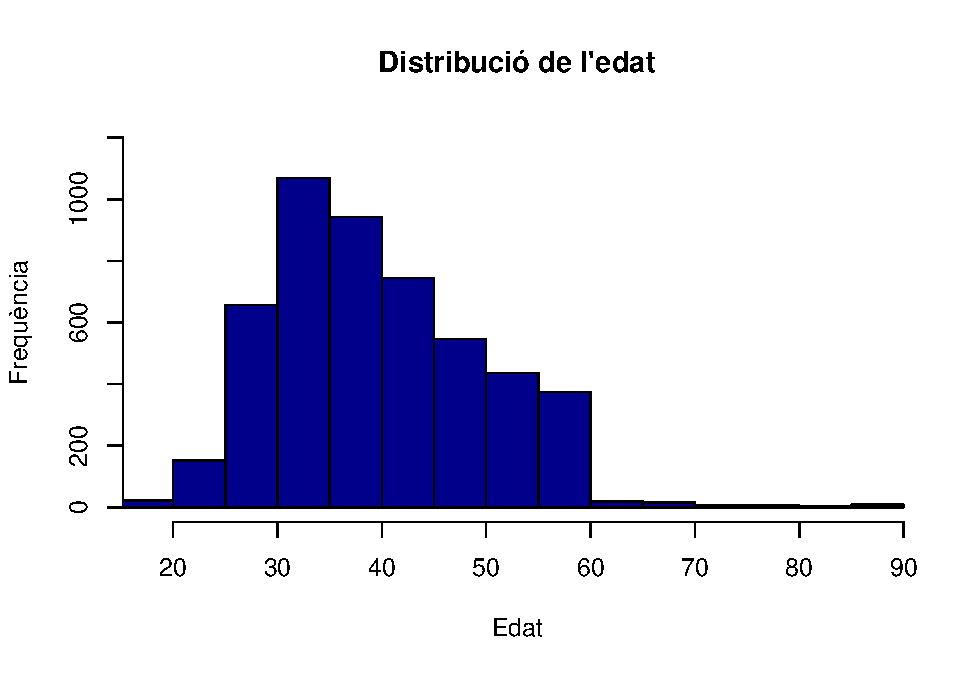
\includegraphics{Entrega-1_files/figure-latex/unnamed-chunk-3-1.pdf}

Agruparem en quatre noves categories: Jove{[}0,25{]},
Jove-Adult{[}26,45{]}, Adult{[}46,65{]}, Gran{[}+66{]}.

Realitzem aquesta distinció pels següents motius:

\begin{itemize}
\item
  Jove: No solen tenir gaire poder adquisitiu propi
\item
  Jove-Adult: És quan s'acostumen a fer més plans de futur i a tenir més
  capacitat econòmica
\item
  Adult: Solen ser persones amb una vida estable i sense gaires canvis
  econòmics grans
\item
  Gran: Persones amb la vida feta, sense canvis econòmics (Com que
  l'edat més gran registrada és 88 anys, entendrem que no tenim
  outliers)
\end{itemize}

La variable passarà a ser categòrica.

\begin{Shaded}
\begin{Highlighting}[]
\NormalTok{df}\SpecialCharTok{$}\NormalTok{age\_num }\OtherTok{\textless{}{-}}\NormalTok{ df}\SpecialCharTok{$}\NormalTok{age}
\NormalTok{df}\SpecialCharTok{$}\NormalTok{age }\OtherTok{\textless{}{-}} \FunctionTok{cut}\NormalTok{(df}\SpecialCharTok{$}\NormalTok{age, }
              \AttributeTok{breaks =} \FunctionTok{c}\NormalTok{(}\DecValTok{0}\NormalTok{, }\DecValTok{25}\NormalTok{, }\DecValTok{45}\NormalTok{, }\DecValTok{65}\NormalTok{, }\FunctionTok{max}\NormalTok{(df}\SpecialCharTok{$}\NormalTok{age)),}
              \AttributeTok{labels =} \FunctionTok{c}\NormalTok{(}\StringTok{"Jove"}\NormalTok{, }\StringTok{"Jove{-}Adult"}\NormalTok{, }\StringTok{"Adult"}\NormalTok{, }\StringTok{"Gran"}\NormalTok{))}
\NormalTok{df}\SpecialCharTok{$}\NormalTok{age }\OtherTok{\textless{}{-}} \FunctionTok{as.factor}\NormalTok{(df}\SpecialCharTok{$}\NormalTok{age)}
\end{Highlighting}
\end{Shaded}

\begin{Shaded}
\begin{Highlighting}[]
\FunctionTok{pie}\NormalTok{(}\FunctionTok{table}\NormalTok{(df}\SpecialCharTok{$}\NormalTok{age),}
        \AttributeTok{col =} \FunctionTok{c}\NormalTok{(}\StringTok{"mistyrose2"}\NormalTok{, }\StringTok{"darkolivegreen3"}\NormalTok{, }\StringTok{"khaki2"}\NormalTok{, }\StringTok{"azure2"}\NormalTok{),}
        \AttributeTok{main =} \StringTok{"Distribució d\textquotesingle{}edats agrupades"}\NormalTok{)}
\FunctionTok{legend}\NormalTok{(}\StringTok{"right"}\NormalTok{, }\AttributeTok{fill =} \FunctionTok{c}\NormalTok{(}\StringTok{"mistyrose2"}\NormalTok{, }\StringTok{"darkolivegreen3"}\NormalTok{, }\StringTok{"khaki2"}\NormalTok{, }\StringTok{"azure2"}\NormalTok{) , }\AttributeTok{legend =} \FunctionTok{paste}\NormalTok{(}\DecValTok{100}\SpecialCharTok{*}\FunctionTok{prop.table}\NormalTok{(}\FunctionTok{table}\NormalTok{(df}\SpecialCharTok{$}\NormalTok{age)), }\StringTok{"\%"}\NormalTok{))}
\end{Highlighting}
\end{Shaded}

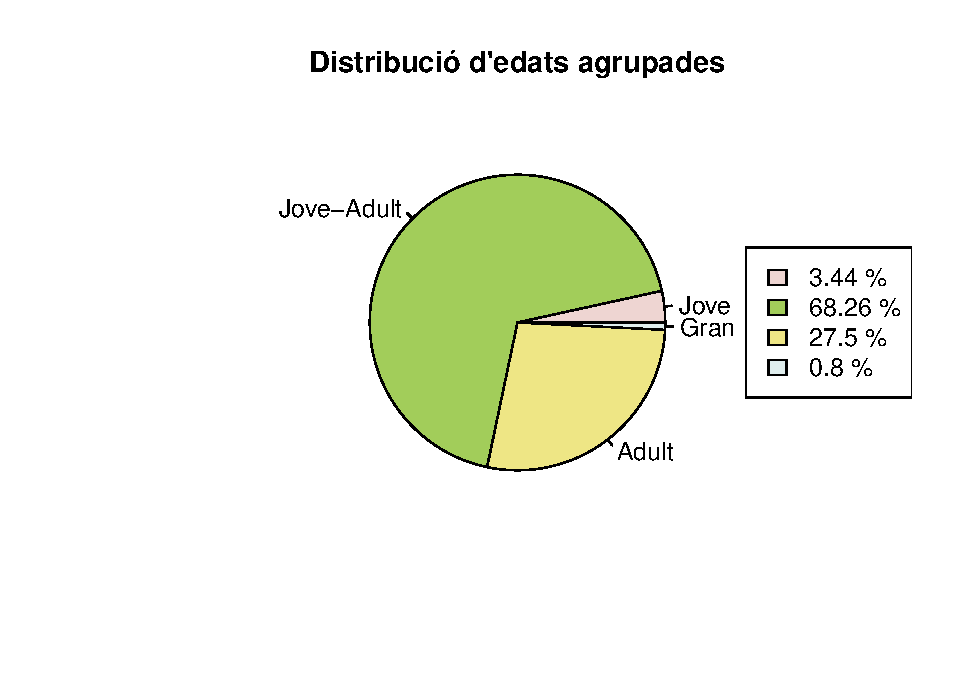
\includegraphics{Entrega-1_files/figure-latex/unnamed-chunk-5-1.pdf}

\hypertarget{job}{%
\paragraph{Job}\label{job}}

\begin{Shaded}
\begin{Highlighting}[]
\FunctionTok{barplot}\NormalTok{(}\DecValTok{100}\SpecialCharTok{*}\FunctionTok{prop.table}\NormalTok{(}\FunctionTok{table}\NormalTok{(df}\SpecialCharTok{$}\NormalTok{job)),}
        \AttributeTok{ylim =} \FunctionTok{c}\NormalTok{(}\DecValTok{0}\NormalTok{, }\DecValTok{30}\NormalTok{),}
        \AttributeTok{col =} \StringTok{"blue4"}\NormalTok{,}
        \AttributeTok{main =} \StringTok{"Distribució de treball"}\NormalTok{,}
        \AttributeTok{ylab =} \StringTok{"Proporció"}\NormalTok{,}
        \AttributeTok{las =} \DecValTok{2}\NormalTok{)}
\end{Highlighting}
\end{Shaded}

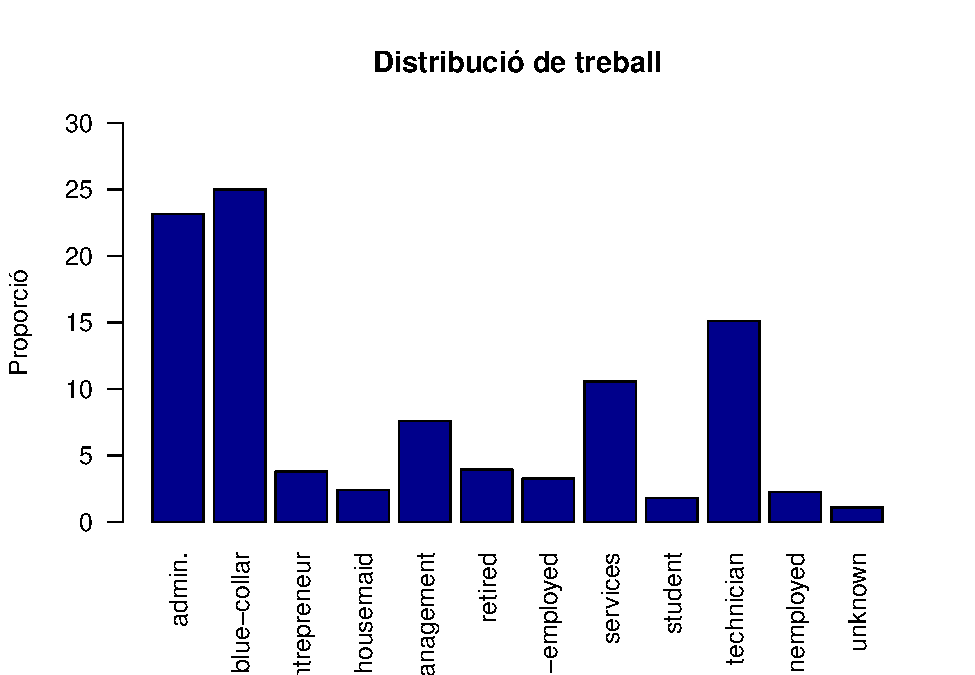
\includegraphics{Entrega-1_files/figure-latex/unnamed-chunk-6-1.pdf}

Les categories ``retired'', ``unemployed'', ``student'' i ``housemaid''
passaran a ser ``unemployed'', ja que tenim en compte que són persones
que no cotitzen.

Els ``enterpeneur'' passaran a ser ``self-employed''. vector indicating
the indexes of the quantitative supplementary variables

\begin{Shaded}
\begin{Highlighting}[]
\NormalTok{df}\SpecialCharTok{$}\NormalTok{job }\OtherTok{\textless{}{-}} \FunctionTok{as.character}\NormalTok{(df}\SpecialCharTok{$}\NormalTok{job)}
\NormalTok{df}\SpecialCharTok{$}\NormalTok{job }\OtherTok{\textless{}{-}} \FunctionTok{ifelse}\NormalTok{(df}\SpecialCharTok{$}\NormalTok{job }\SpecialCharTok{\%in\%} \FunctionTok{c}\NormalTok{(}\StringTok{"retired"}\NormalTok{, }\StringTok{"unemployed"}\NormalTok{, }\StringTok{"student"}\NormalTok{, }\StringTok{"housemaid"}\NormalTok{), }\StringTok{"unemployed"}\NormalTok{, df}\SpecialCharTok{$}\NormalTok{job)}
\NormalTok{df}\SpecialCharTok{$}\NormalTok{job }\OtherTok{\textless{}{-}} \FunctionTok{ifelse}\NormalTok{(df}\SpecialCharTok{$}\NormalTok{job }\SpecialCharTok{==} \StringTok{"entrepreneur"}\NormalTok{, }\StringTok{"self{-}employed"}\NormalTok{, df}\SpecialCharTok{$}\NormalTok{job)}
\NormalTok{df}\SpecialCharTok{$}\NormalTok{job }\OtherTok{\textless{}{-}} \FunctionTok{as.factor}\NormalTok{(df}\SpecialCharTok{$}\NormalTok{job)}
\end{Highlighting}
\end{Shaded}

\begin{Shaded}
\begin{Highlighting}[]
\FunctionTok{barplot}\NormalTok{(}\DecValTok{100}\SpecialCharTok{*}\FunctionTok{prop.table}\NormalTok{(}\FunctionTok{table}\NormalTok{(df}\SpecialCharTok{$}\NormalTok{job)),}
        \AttributeTok{ylim =} \FunctionTok{c}\NormalTok{(}\DecValTok{0}\NormalTok{, }\DecValTok{30}\NormalTok{),}
        \AttributeTok{col =} \StringTok{"blue4"}\NormalTok{,}
        \AttributeTok{main =} \StringTok{"Distribució de treball agrupada"}\NormalTok{,}
        \AttributeTok{ylab =} \StringTok{"Proporció"}\NormalTok{,}
        \AttributeTok{las =} \DecValTok{2}\NormalTok{)}
\end{Highlighting}
\end{Shaded}

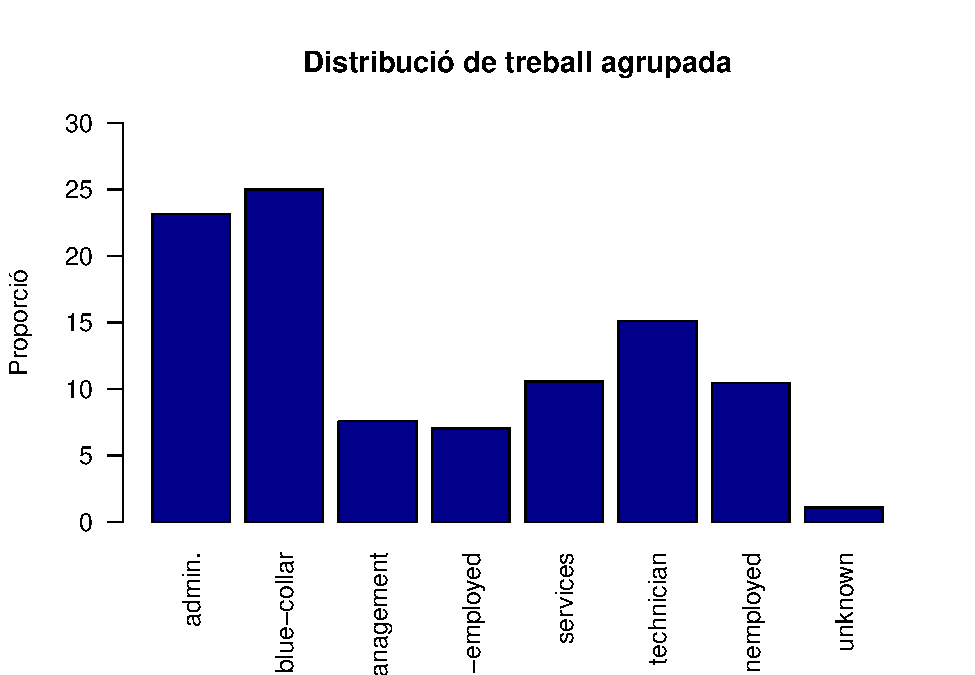
\includegraphics{Entrega-1_files/figure-latex/unnamed-chunk-8-1.pdf}

\hypertarget{marital}{%
\paragraph{Marital}\label{marital}}

\begin{Shaded}
\begin{Highlighting}[]
\FunctionTok{barplot}\NormalTok{(}\DecValTok{100}\SpecialCharTok{*}\FunctionTok{prop.table}\NormalTok{(}\FunctionTok{table}\NormalTok{(df}\SpecialCharTok{$}\NormalTok{marital)),}
        \AttributeTok{ylim =} \FunctionTok{c}\NormalTok{(}\DecValTok{0}\NormalTok{, }\DecValTok{70}\NormalTok{),}
        \AttributeTok{main =} \StringTok{"Distribució de l\textquotesingle{}estat civil"}\NormalTok{, }
        \AttributeTok{ylab =} \StringTok{"Proporció"}\NormalTok{, }
        \AttributeTok{col =} \StringTok{"blue4"}\NormalTok{)}
\end{Highlighting}
\end{Shaded}

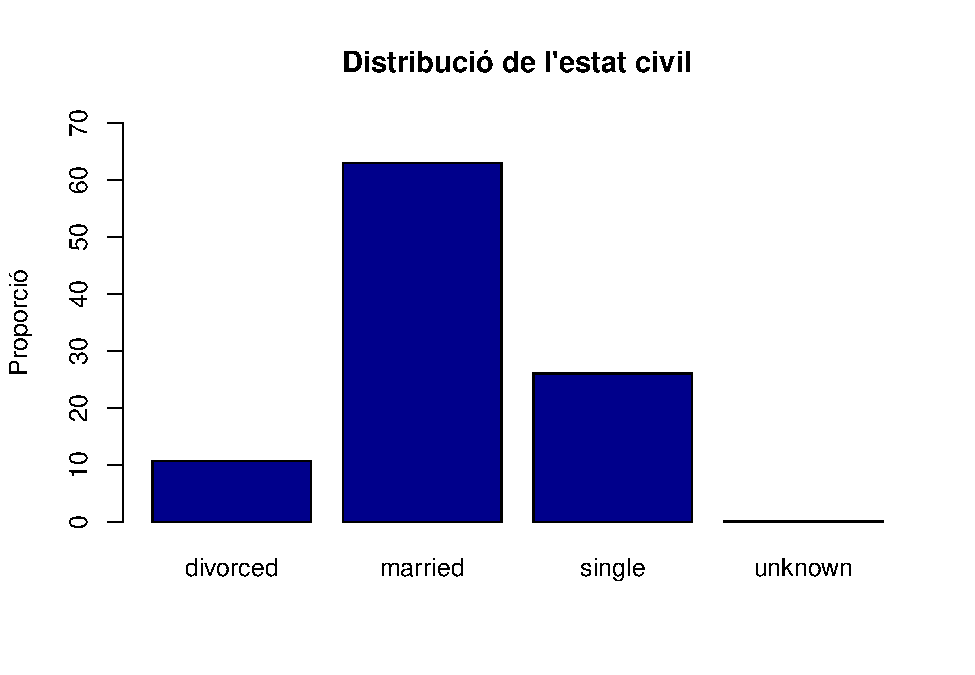
\includegraphics{Entrega-1_files/figure-latex/unnamed-chunk-9-1.pdf}

\hypertarget{education}{%
\paragraph{Education}\label{education}}

\begin{Shaded}
\begin{Highlighting}[]
\FunctionTok{barplot}\NormalTok{(}\DecValTok{100}\SpecialCharTok{*}\FunctionTok{prop.table}\NormalTok{(}\FunctionTok{table}\NormalTok{(df}\SpecialCharTok{$}\NormalTok{education)),}
        \AttributeTok{ylim =} \FunctionTok{c}\NormalTok{(}\DecValTok{0}\NormalTok{, }\DecValTok{30}\NormalTok{),}
        \AttributeTok{col =} \StringTok{"blue4"}\NormalTok{,}
        \AttributeTok{main =} \StringTok{"Nivell d\textquotesingle{}educació"}\NormalTok{,}
        \AttributeTok{ylab =} \StringTok{"Proporció"}\NormalTok{,}
        \AttributeTok{las =} \DecValTok{2}\NormalTok{)}
\end{Highlighting}
\end{Shaded}

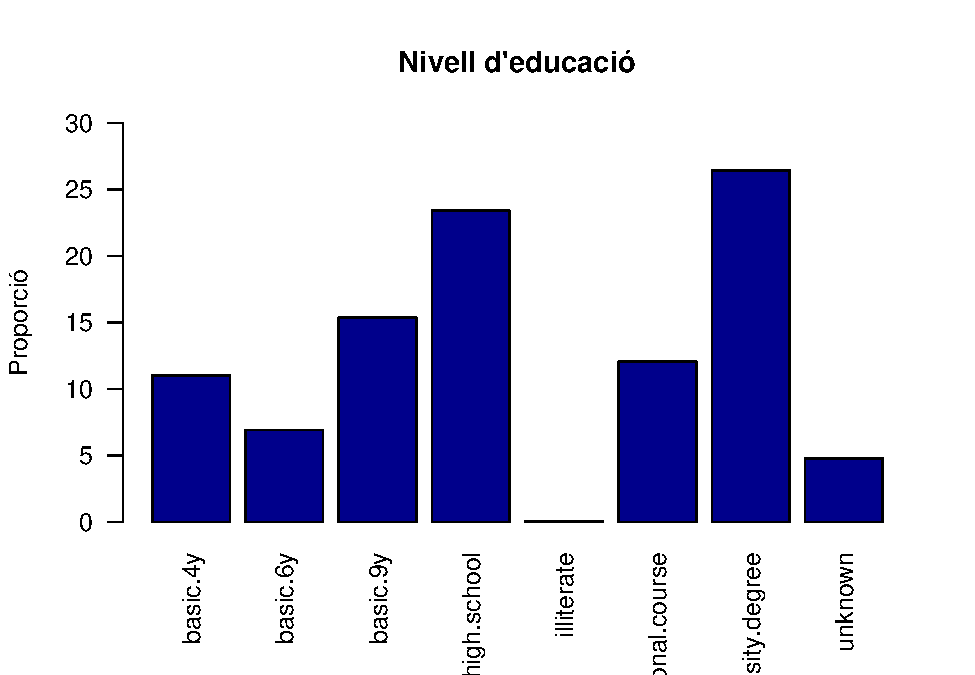
\includegraphics{Entrega-1_files/figure-latex/unnamed-chunk-10-1.pdf}

Les categories ``basic.4y'', ``basic.6y'', ``basic.9y'' passaran a ser
``basic'', ja que no aporta informació saber quin nivell de ``basic''
tenen.

\begin{Shaded}
\begin{Highlighting}[]
\NormalTok{df}\SpecialCharTok{$}\NormalTok{education }\OtherTok{\textless{}{-}} \FunctionTok{as.character}\NormalTok{(df}\SpecialCharTok{$}\NormalTok{education)}
\NormalTok{df}\SpecialCharTok{$}\NormalTok{education }\OtherTok{\textless{}{-}} \FunctionTok{ifelse}\NormalTok{(df}\SpecialCharTok{$}\NormalTok{education }\SpecialCharTok{\%in\%} \FunctionTok{c}\NormalTok{(}\StringTok{"basic.4y"}\NormalTok{, }\StringTok{"basic.6y"}\NormalTok{, }\StringTok{"basic.9y"}\NormalTok{), }\StringTok{"basic"}\NormalTok{, df}\SpecialCharTok{$}\NormalTok{education)}
\NormalTok{df}\SpecialCharTok{$}\NormalTok{education }\OtherTok{\textless{}{-}} \FunctionTok{as.factor}\NormalTok{(df}\SpecialCharTok{$}\NormalTok{education)}
\end{Highlighting}
\end{Shaded}

\begin{Shaded}
\begin{Highlighting}[]
\FunctionTok{barplot}\NormalTok{(}\DecValTok{100}\SpecialCharTok{*}\FunctionTok{prop.table}\NormalTok{(}\FunctionTok{table}\NormalTok{(df}\SpecialCharTok{$}\NormalTok{education)),}
        \AttributeTok{ylim =} \FunctionTok{c}\NormalTok{(}\DecValTok{0}\NormalTok{, }\DecValTok{35}\NormalTok{),}
        \AttributeTok{col =} \StringTok{"blue4"}\NormalTok{,}
        \AttributeTok{main =} \StringTok{"Distribució del nivell d\textquotesingle{}educació agrupada"}\NormalTok{,}
        \AttributeTok{ylab =} \StringTok{"Proporció"}\NormalTok{,}
        \AttributeTok{las =} \DecValTok{2}\NormalTok{)}
\end{Highlighting}
\end{Shaded}

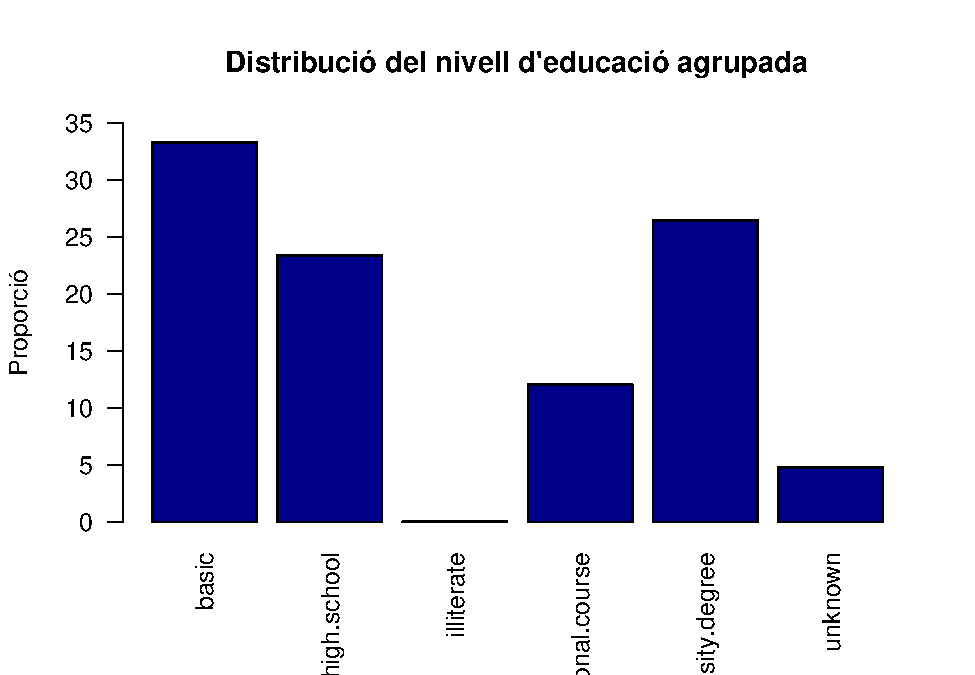
\includegraphics{Entrega-1_files/figure-latex/unnamed-chunk-12-1.pdf}

\hypertarget{housing}{%
\paragraph{Housing}\label{housing}}

\begin{Shaded}
\begin{Highlighting}[]
\FunctionTok{pie}\NormalTok{(}\FunctionTok{prop.table}\NormalTok{(}\FunctionTok{table}\NormalTok{(df}\SpecialCharTok{$}\NormalTok{housing)),}
        \AttributeTok{col =} \FunctionTok{c}\NormalTok{(}\StringTok{"brown3"}\NormalTok{, }\StringTok{"yellow2"}\NormalTok{, }\StringTok{"green3"}\NormalTok{),}
        \AttributeTok{main =} \StringTok{"Distribució de hipotèques"}\NormalTok{)}
\FunctionTok{legend}\NormalTok{(}\StringTok{"right"}\NormalTok{, }\AttributeTok{fill =} \FunctionTok{c}\NormalTok{(}\StringTok{"brown3"}\NormalTok{, }\StringTok{"yellow2"}\NormalTok{, }\StringTok{"green3"}\NormalTok{) , }\AttributeTok{legend =} \FunctionTok{paste}\NormalTok{(}\DecValTok{100}\SpecialCharTok{*}\FunctionTok{prop.table}\NormalTok{(}\FunctionTok{table}\NormalTok{(df}\SpecialCharTok{$}\NormalTok{housing)), }\StringTok{"\%"}\NormalTok{))}
\end{Highlighting}
\end{Shaded}

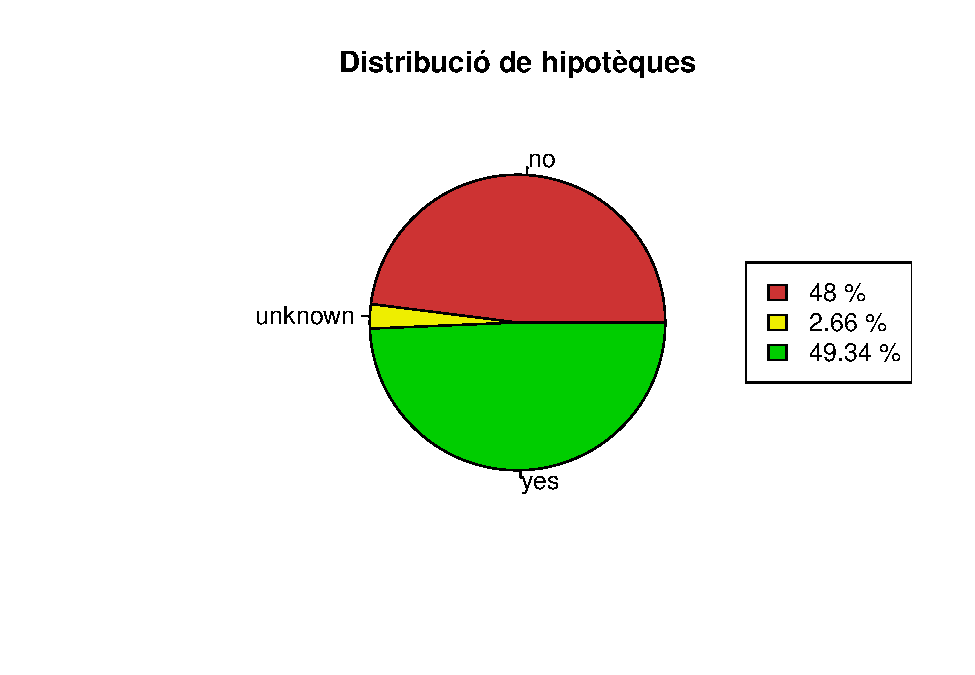
\includegraphics{Entrega-1_files/figure-latex/unnamed-chunk-13-1.pdf}

\hypertarget{loan}{%
\paragraph{Loan}\label{loan}}

\begin{Shaded}
\begin{Highlighting}[]
\FunctionTok{pie}\NormalTok{(}\FunctionTok{prop.table}\NormalTok{(}\FunctionTok{table}\NormalTok{(df}\SpecialCharTok{$}\NormalTok{loan)),}
        \AttributeTok{col =} \FunctionTok{c}\NormalTok{(}\StringTok{"brown3"}\NormalTok{, }\StringTok{"yellow2"}\NormalTok{, }\StringTok{"green3"}\NormalTok{),}
        \AttributeTok{main =} \StringTok{"Distribució de préstecs"}\NormalTok{)}
\FunctionTok{legend}\NormalTok{(}\StringTok{"right"}\NormalTok{, }\AttributeTok{fill =} \FunctionTok{c}\NormalTok{(}\StringTok{"brown3"}\NormalTok{, }\StringTok{"yellow2"}\NormalTok{, }\StringTok{"green3"}\NormalTok{) , }\AttributeTok{legend =} \FunctionTok{paste}\NormalTok{(}\DecValTok{100}\SpecialCharTok{*}\FunctionTok{prop.table}\NormalTok{(}\FunctionTok{table}\NormalTok{(df}\SpecialCharTok{$}\NormalTok{loan)), }\StringTok{"\%"}\NormalTok{))}
\end{Highlighting}
\end{Shaded}

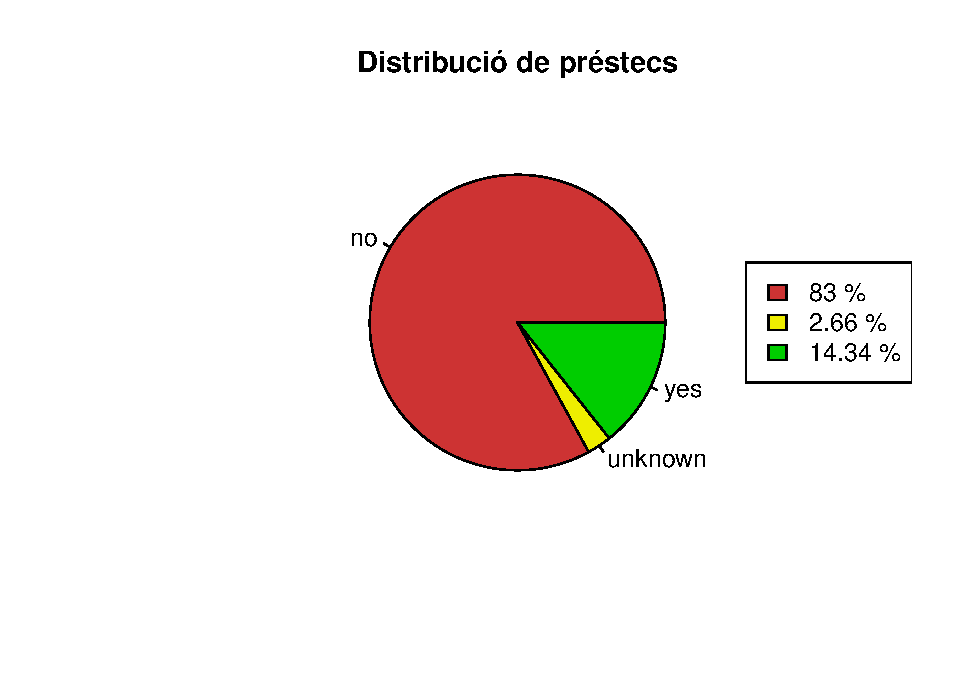
\includegraphics{Entrega-1_files/figure-latex/unnamed-chunk-14-1.pdf}

\hypertarget{contact}{%
\paragraph{Contact}\label{contact}}

\begin{Shaded}
\begin{Highlighting}[]
\FunctionTok{pie}\NormalTok{(}\FunctionTok{table}\NormalTok{(df}\SpecialCharTok{$}\NormalTok{contact),}
        \AttributeTok{col =} \FunctionTok{c}\NormalTok{(}\StringTok{"darkolivegreen3"}\NormalTok{, }\StringTok{"khaki2"}\NormalTok{),}
        \AttributeTok{main =} \StringTok{"Distribució de forma de comunicació"}\NormalTok{)}
\FunctionTok{legend}\NormalTok{(}\StringTok{"right"}\NormalTok{, }\AttributeTok{fill =} \FunctionTok{c}\NormalTok{(}\StringTok{"darkolivegreen3"}\NormalTok{, }\StringTok{"khaki2"}\NormalTok{) , }\AttributeTok{legend =} \FunctionTok{paste}\NormalTok{(}\DecValTok{100}\SpecialCharTok{*}\FunctionTok{prop.table}\NormalTok{(}\FunctionTok{table}\NormalTok{(df}\SpecialCharTok{$}\NormalTok{contact)), }\StringTok{"\%"}\NormalTok{))}
\end{Highlighting}
\end{Shaded}

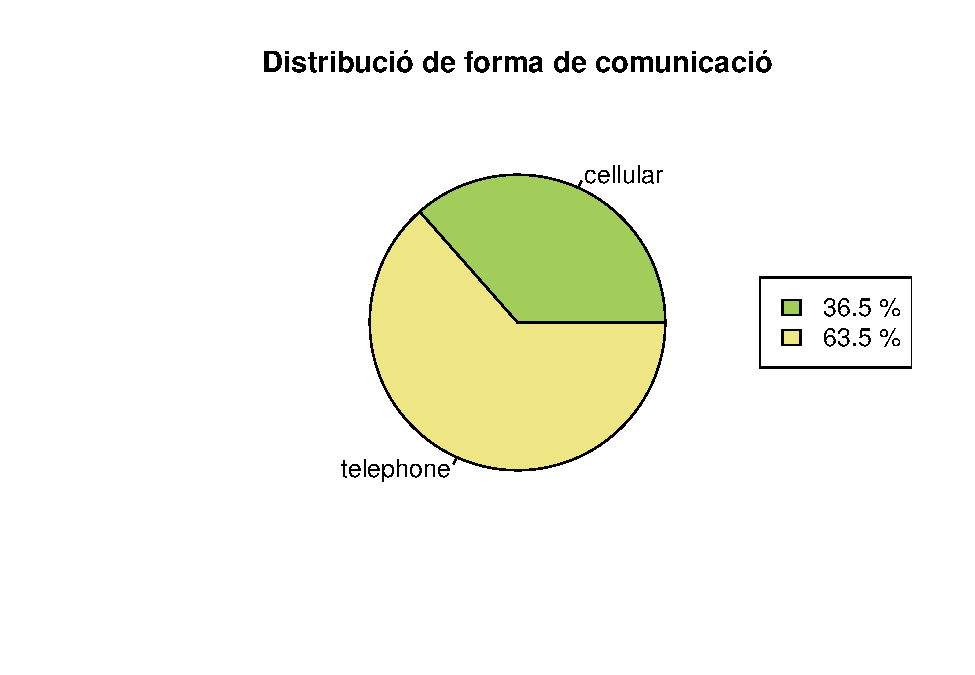
\includegraphics{Entrega-1_files/figure-latex/unnamed-chunk-15-1.pdf}

\hypertarget{month}{%
\paragraph{Month}\label{month}}

\begin{Shaded}
\begin{Highlighting}[]
\NormalTok{mesos }\OtherTok{\textless{}{-}} \FunctionTok{c}\NormalTok{(}\StringTok{"jan"}\NormalTok{, }\StringTok{"feb"}\NormalTok{, }\StringTok{"mar"}\NormalTok{, }\StringTok{"apr"}\NormalTok{, }\StringTok{"may"}\NormalTok{, }\StringTok{"jun"}\NormalTok{, }\StringTok{"jul"}\NormalTok{, }\StringTok{"aug"}\NormalTok{, }\StringTok{"sep"}\NormalTok{, }\StringTok{"oct"}\NormalTok{, }\StringTok{"nov"}\NormalTok{, }\StringTok{"dec"}\NormalTok{)}

\NormalTok{df}\SpecialCharTok{$}\NormalTok{month }\OtherTok{\textless{}{-}} \FunctionTok{factor}\NormalTok{(df}\SpecialCharTok{$}\NormalTok{month, }\AttributeTok{levels =}\NormalTok{ mesos)}

\FunctionTok{barplot}\NormalTok{(}\FunctionTok{table}\NormalTok{(df}\SpecialCharTok{$}\NormalTok{month),}
        \AttributeTok{ylim =} \FunctionTok{c}\NormalTok{(}\DecValTok{0}\NormalTok{, }\DecValTok{3500}\NormalTok{),}
        \AttributeTok{col =} \StringTok{"blue4"}\NormalTok{,}
        \AttributeTok{ylab =} \StringTok{"Freqüència"}\NormalTok{,}
        \AttributeTok{main =} \StringTok{"Distribució de les trucades per mesos"}\NormalTok{)}
\end{Highlighting}
\end{Shaded}

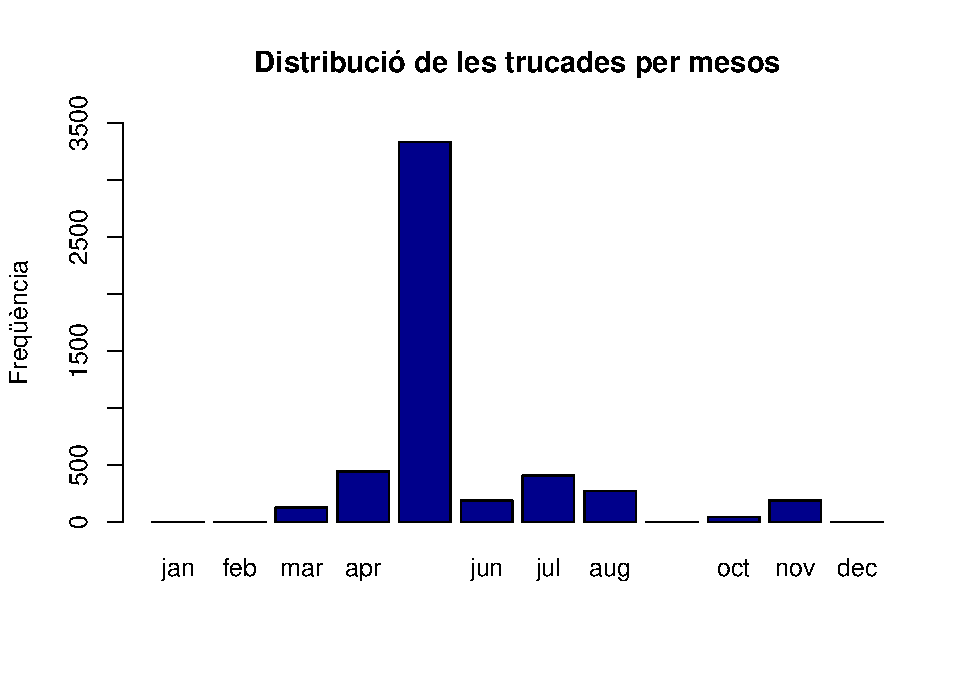
\includegraphics{Entrega-1_files/figure-latex/unnamed-chunk-16-1.pdf}

\hypertarget{day-of-the-week}{%
\paragraph{Day of the week}\label{day-of-the-week}}

\begin{Shaded}
\begin{Highlighting}[]
\NormalTok{days }\OtherTok{\textless{}{-}} \FunctionTok{c}\NormalTok{(}\StringTok{"mon"}\NormalTok{, }\StringTok{"tue"}\NormalTok{, }\StringTok{"wed"}\NormalTok{, }\StringTok{"thu"}\NormalTok{, }\StringTok{"fri"}\NormalTok{, }\StringTok{"sat"}\NormalTok{, }\StringTok{"sun"}\NormalTok{)}

\NormalTok{df}\SpecialCharTok{$}\NormalTok{day\_of\_week }\OtherTok{\textless{}{-}} \FunctionTok{factor}\NormalTok{(df}\SpecialCharTok{$}\NormalTok{day\_of\_week, }\AttributeTok{levels =}\NormalTok{ days)}

\FunctionTok{barplot}\NormalTok{(}\FunctionTok{table}\NormalTok{(df}\SpecialCharTok{$}\NormalTok{day\_of\_week),}
        \AttributeTok{ylim =} \FunctionTok{c}\NormalTok{(}\DecValTok{0}\NormalTok{, }\DecValTok{1400}\NormalTok{),}
        \AttributeTok{col =} \StringTok{"blue4"}\NormalTok{,}
        \AttributeTok{ylab =} \StringTok{"Freqüència"}\NormalTok{,}
        \AttributeTok{main =} \StringTok{"Distribució de trucades per dies"}\NormalTok{)}
\end{Highlighting}
\end{Shaded}

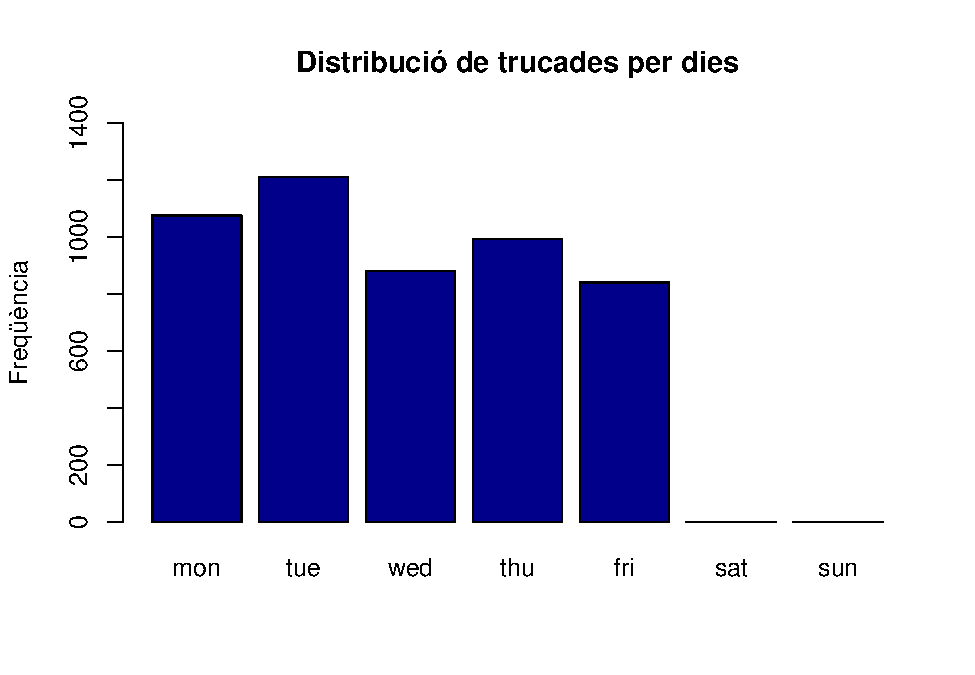
\includegraphics{Entrega-1_files/figure-latex/unnamed-chunk-17-1.pdf}

\hypertarget{duration}{%
\paragraph{Duration}\label{duration}}

\begin{Shaded}
\begin{Highlighting}[]
\FunctionTok{hist}\NormalTok{(df}\SpecialCharTok{$}\NormalTok{duration,}
     \AttributeTok{col =} \StringTok{"blue4"}\NormalTok{,}
     \AttributeTok{xlim =} \FunctionTok{c}\NormalTok{(}\FunctionTok{min}\NormalTok{(df}\SpecialCharTok{$}\NormalTok{duration),}
              \FunctionTok{max}\NormalTok{(df}\SpecialCharTok{$}\NormalTok{duration)),}
              \AttributeTok{ylim =} \FunctionTok{c}\NormalTok{(}\DecValTok{0}\NormalTok{, }\DecValTok{3500}\NormalTok{),}
              \AttributeTok{main =} \StringTok{"Distribució de la duració de les trucades"}\NormalTok{, }
              \AttributeTok{xlab =} \StringTok{"Duració (segons)"}\NormalTok{, }
              \AttributeTok{ylab =} \StringTok{"Frequència"}\NormalTok{)}
\end{Highlighting}
\end{Shaded}

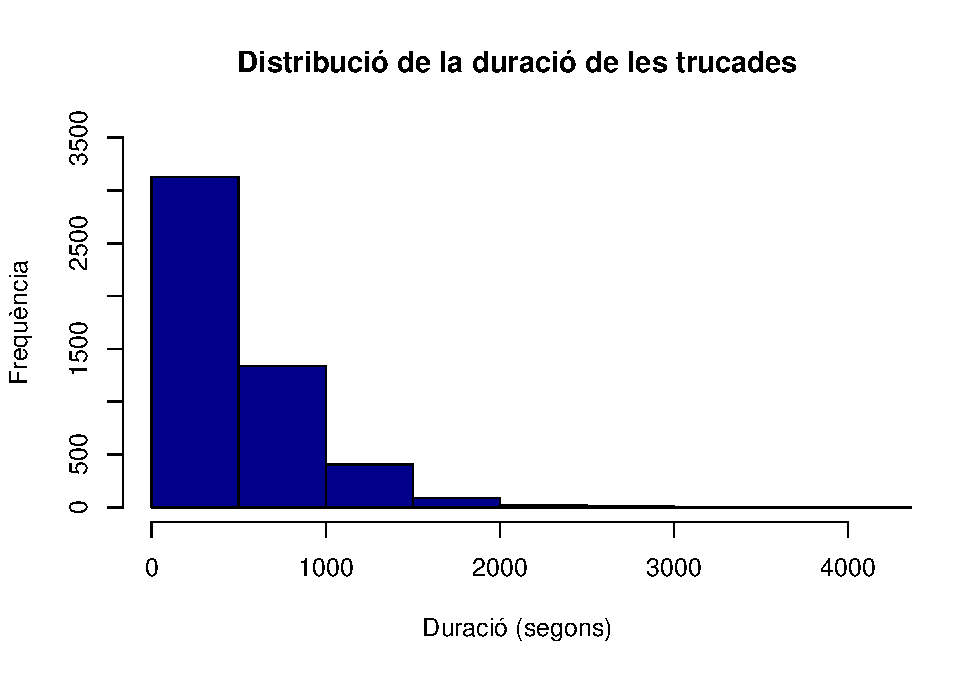
\includegraphics{Entrega-1_files/figure-latex/unnamed-chunk-18-1.pdf}

\hypertarget{campaign}{%
\paragraph{Campaign}\label{campaign}}

\begin{Shaded}
\begin{Highlighting}[]
\FunctionTok{hist}\NormalTok{(df}\SpecialCharTok{$}\NormalTok{campaign,}
     \AttributeTok{col =} \StringTok{"blue4"}\NormalTok{,}
              \AttributeTok{ylim =} \FunctionTok{c}\NormalTok{(}\DecValTok{0}\NormalTok{, }\DecValTok{4000}\NormalTok{),}
              \AttributeTok{main =} \StringTok{"Distribució dels contactes per client de la campanya actual"}\NormalTok{, }
              \AttributeTok{xlab =} \StringTok{"Número de contactes"}\NormalTok{, }
              \AttributeTok{ylab =} \StringTok{"Frequència"}\NormalTok{)}
\end{Highlighting}
\end{Shaded}

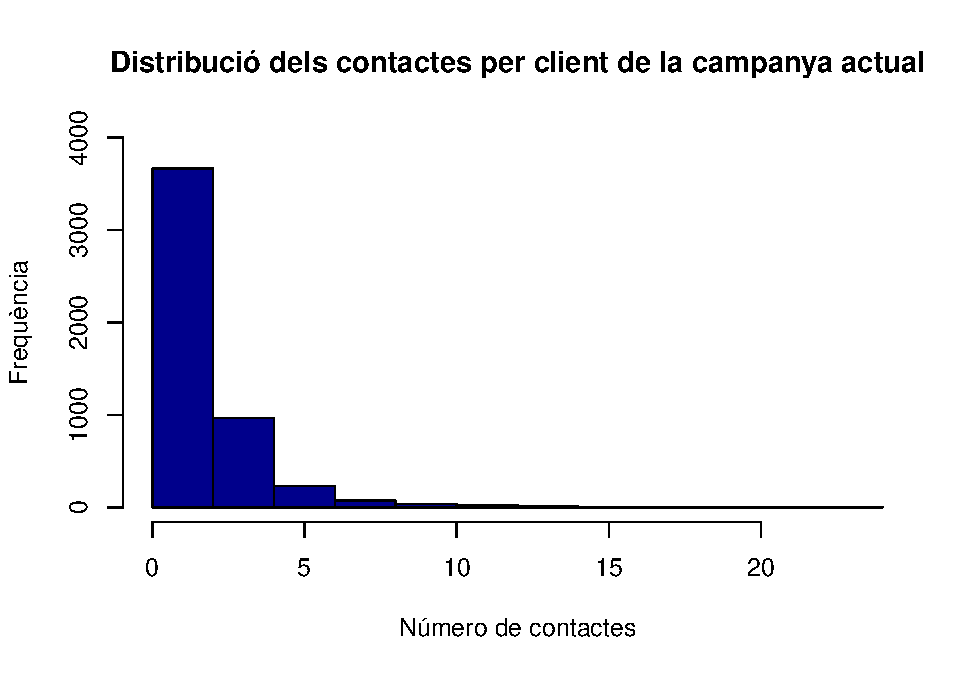
\includegraphics{Entrega-1_files/figure-latex/unnamed-chunk-19-1.pdf}

\hypertarget{pdays}{%
\paragraph{Pdays}\label{pdays}}

\begin{Shaded}
\begin{Highlighting}[]
\NormalTok{pdays\_aux }\OtherTok{\textless{}{-}} \FunctionTok{subset}\NormalTok{(df}\SpecialCharTok{$}\NormalTok{pdays, df}\SpecialCharTok{$}\NormalTok{pdays }\SpecialCharTok{!=} \DecValTok{999}\NormalTok{)}
\FunctionTok{hist}\NormalTok{(pdays\_aux,}
     \AttributeTok{col =} \StringTok{"blue4"}\NormalTok{,}
              \AttributeTok{ylim =} \FunctionTok{c}\NormalTok{(}\DecValTok{0}\NormalTok{, }\DecValTok{30}\NormalTok{),}
              \AttributeTok{main =} \StringTok{"Distribució dels dies entre contactes de diferents campanyes"}\NormalTok{, }
              \AttributeTok{xlab =} \StringTok{"Número de dies"}\NormalTok{, }
              \AttributeTok{ylab =} \StringTok{"Frequència"}\NormalTok{)}
\end{Highlighting}
\end{Shaded}

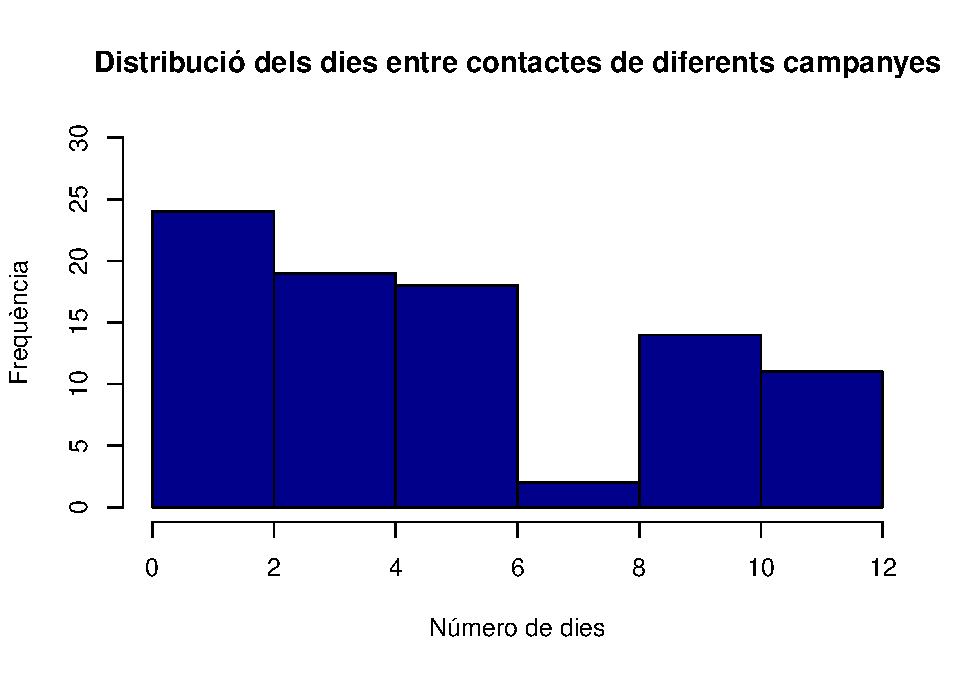
\includegraphics{Entrega-1_files/figure-latex/unnamed-chunk-20-1.pdf}

\hypertarget{previous}{%
\paragraph{Previous}\label{previous}}

\begin{Shaded}
\begin{Highlighting}[]
\FunctionTok{hist}\NormalTok{(df}\SpecialCharTok{$}\NormalTok{previous,}
     \AttributeTok{col =} \StringTok{"blue4"}\NormalTok{,}
              \AttributeTok{ylim =} \FunctionTok{c}\NormalTok{(}\DecValTok{0}\NormalTok{, }\DecValTok{5000}\NormalTok{),}
              \AttributeTok{main =} \StringTok{"Distribució del número de contactes anteriors (diferents campanyes)"}\NormalTok{, }
              \AttributeTok{xlab =} \StringTok{"Número de contactes"}\NormalTok{, }
              \AttributeTok{ylab =} \StringTok{"Frequència"}\NormalTok{)}
\end{Highlighting}
\end{Shaded}

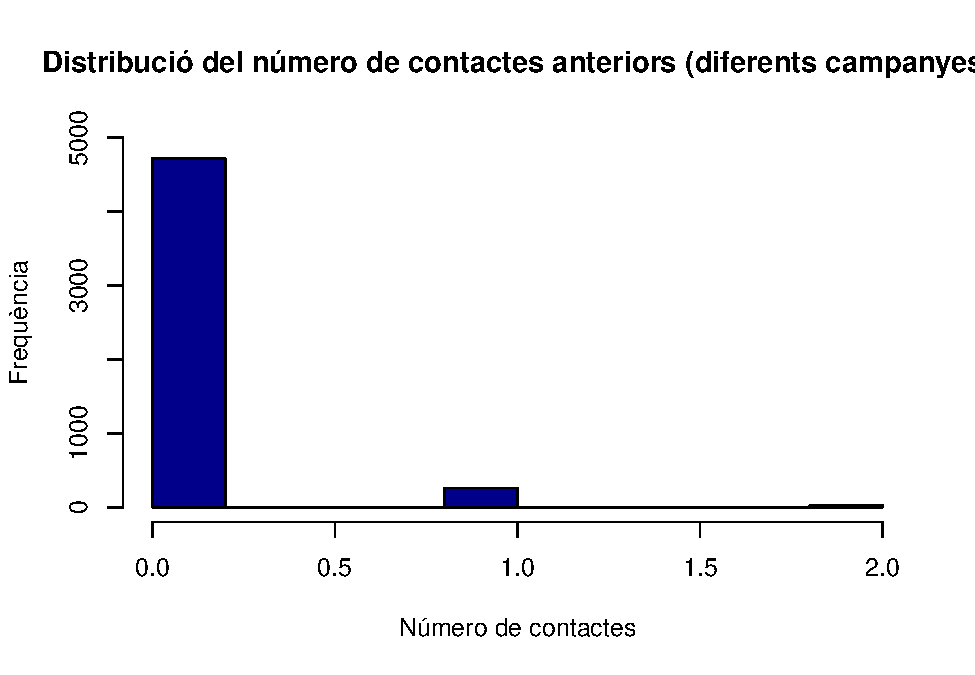
\includegraphics{Entrega-1_files/figure-latex/unnamed-chunk-21-1.pdf}

Ho passem a dos valors possibles: No{[}0{]} Yes{[}+1{]}.

La variable passarà a ser categòrica.

\begin{Shaded}
\begin{Highlighting}[]
\NormalTok{df }\OtherTok{\textless{}{-}}\NormalTok{ df }\SpecialCharTok{\%\textgreater{}\%} \FunctionTok{mutate}\NormalTok{(}\AttributeTok{previous =} \FunctionTok{ifelse}\NormalTok{(previous }\SpecialCharTok{\textgreater{}=} \DecValTok{1}\NormalTok{, }\StringTok{"Yes"}\NormalTok{ , previous))}
\NormalTok{df }\OtherTok{\textless{}{-}}\NormalTok{ df }\SpecialCharTok{\%\textgreater{}\%} \FunctionTok{mutate}\NormalTok{(}\AttributeTok{previous =} \FunctionTok{ifelse}\NormalTok{(previous }\SpecialCharTok{==} \DecValTok{0}\NormalTok{, }\StringTok{"No"}\NormalTok{ , previous))}
\NormalTok{df}\SpecialCharTok{$}\NormalTok{previous }\OtherTok{\textless{}{-}} \FunctionTok{as.factor}\NormalTok{(df}\SpecialCharTok{$}\NormalTok{previous)}
\end{Highlighting}
\end{Shaded}

\begin{Shaded}
\begin{Highlighting}[]
\FunctionTok{pie}\NormalTok{(}\FunctionTok{table}\NormalTok{(df}\SpecialCharTok{$}\NormalTok{previous), }\AttributeTok{main =} \StringTok{"Distribució unificada de contactes anteriors (diferents campanyes)"}\NormalTok{,}
    \AttributeTok{col =} \FunctionTok{c}\NormalTok{(}\StringTok{"brown3"}\NormalTok{, }\StringTok{"green3"}\NormalTok{))}
\FunctionTok{legend}\NormalTok{(}\StringTok{"right"}\NormalTok{, }\AttributeTok{fill =} \FunctionTok{c}\NormalTok{(}\StringTok{"brown3"}\NormalTok{, }\StringTok{"green3"}\NormalTok{) , }\AttributeTok{legend =} \FunctionTok{paste}\NormalTok{(}\DecValTok{100}\SpecialCharTok{*}\FunctionTok{prop.table}\NormalTok{(}\FunctionTok{table}\NormalTok{(df}\SpecialCharTok{$}\NormalTok{previous)), }\StringTok{"\%"}\NormalTok{))}
\end{Highlighting}
\end{Shaded}

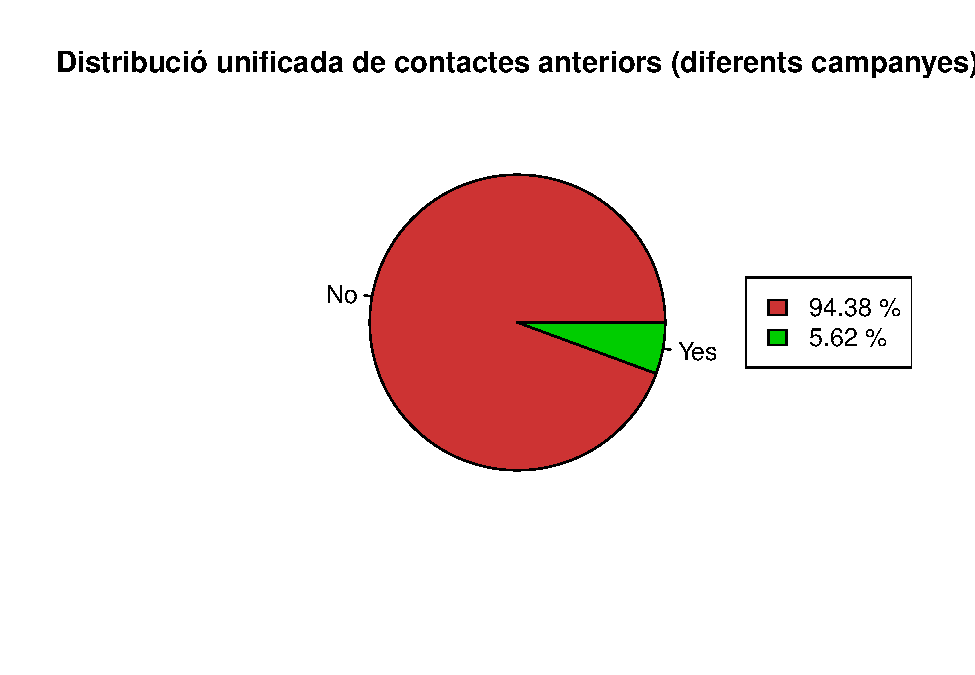
\includegraphics{Entrega-1_files/figure-latex/unnamed-chunk-23-1.pdf}

\hypertarget{poutcome}{%
\paragraph{Poutcome}\label{poutcome}}

\begin{Shaded}
\begin{Highlighting}[]
\FunctionTok{barplot}\NormalTok{(}\FunctionTok{table}\NormalTok{(df}\SpecialCharTok{$}\NormalTok{poutcome),}
        \AttributeTok{ylim =} \FunctionTok{c}\NormalTok{(}\DecValTok{0}\NormalTok{, }\DecValTok{5000}\NormalTok{),}
        \AttributeTok{col =} \StringTok{"blue4"}\NormalTok{,}
        \AttributeTok{ylab =} \StringTok{"Freqüència"}\NormalTok{,}
        \AttributeTok{main =} \StringTok{"Distribució del resultat de campanyes anteriors"}\NormalTok{)}
\end{Highlighting}
\end{Shaded}

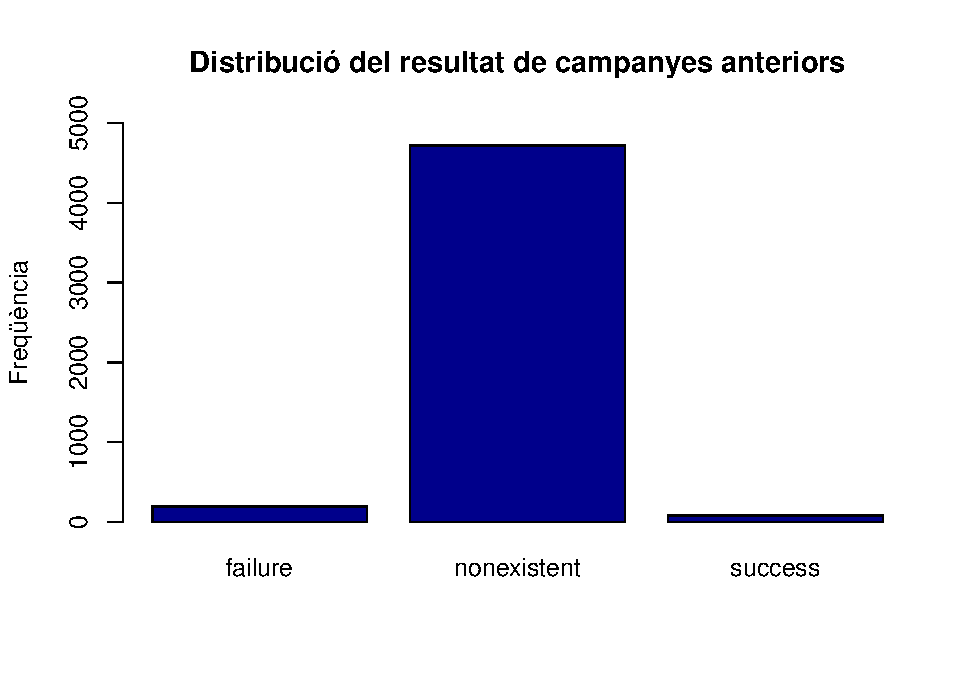
\includegraphics{Entrega-1_files/figure-latex/unnamed-chunk-24-1.pdf}

\hypertarget{employment-variation-rate}{%
\paragraph{Employment variation rate}\label{employment-variation-rate}}

\begin{Shaded}
\begin{Highlighting}[]
\FunctionTok{hist}\NormalTok{(df}\SpecialCharTok{$}\NormalTok{emp.var.rate,}
     \AttributeTok{ylim =} \FunctionTok{c}\NormalTok{(}\DecValTok{0}\NormalTok{, }\DecValTok{3000}\NormalTok{),}
        \AttributeTok{col =} \StringTok{"blue4"}\NormalTok{,}
        \AttributeTok{xlab =} \StringTok{""}\NormalTok{,}
        \AttributeTok{ylab =} \StringTok{"Freqüència"}\NormalTok{,}
        \AttributeTok{main =} \StringTok{"Índex de variació d\textquotesingle{}ocupació"}\NormalTok{)}
\end{Highlighting}
\end{Shaded}

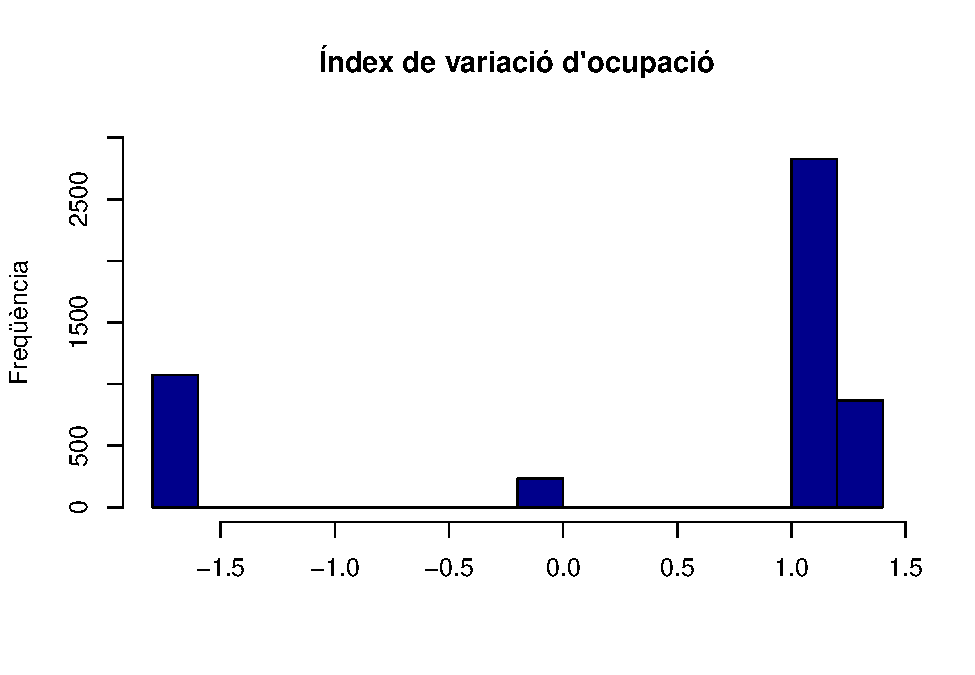
\includegraphics{Entrega-1_files/figure-latex/unnamed-chunk-25-1.pdf}

\hypertarget{consumer-price-index}{%
\paragraph{Consumer price index}\label{consumer-price-index}}

\begin{Shaded}
\begin{Highlighting}[]
\FunctionTok{hist}\NormalTok{(df}\SpecialCharTok{$}\NormalTok{cons.price.idx,}
     \AttributeTok{ylim =} \FunctionTok{c}\NormalTok{(}\DecValTok{0}\NormalTok{, }\DecValTok{3500}\NormalTok{),}
        \AttributeTok{col =} \StringTok{"blue4"}\NormalTok{,}
        \AttributeTok{xlab =} \StringTok{""}\NormalTok{,}
        \AttributeTok{ylab =} \StringTok{"Freqüència"}\NormalTok{,}
        \AttributeTok{main =} \StringTok{"Índex de preus al consumidor"}\NormalTok{)}
\end{Highlighting}
\end{Shaded}

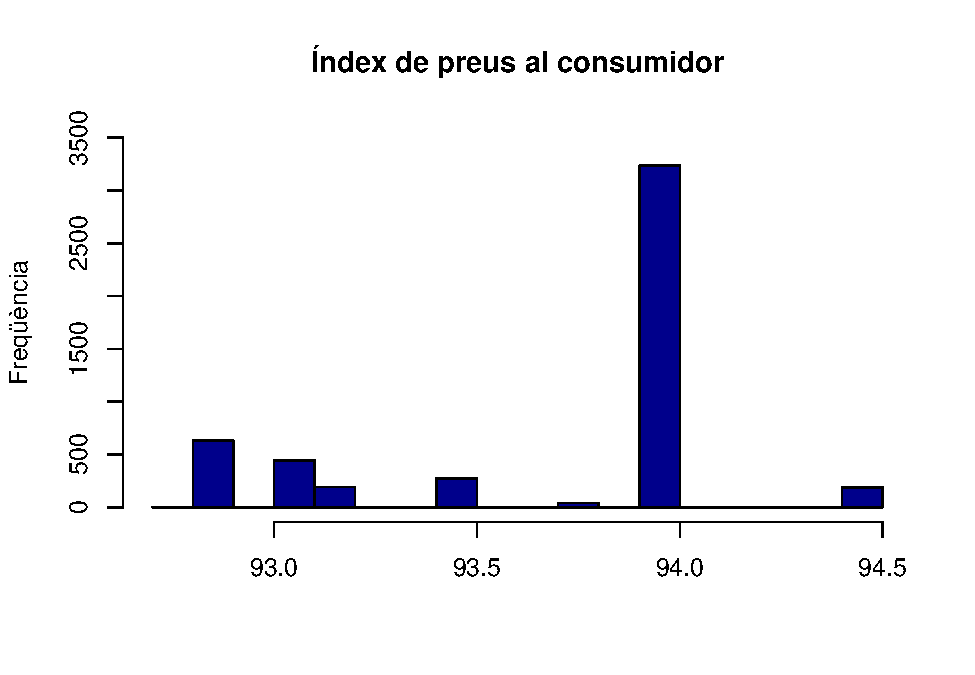
\includegraphics{Entrega-1_files/figure-latex/unnamed-chunk-26-1.pdf}

\hypertarget{consumer-confidence-index}{%
\paragraph{Consumer confidence index}\label{consumer-confidence-index}}

\begin{Shaded}
\begin{Highlighting}[]
\FunctionTok{hist}\NormalTok{(df}\SpecialCharTok{$}\NormalTok{cons.conf.idx,}
     \AttributeTok{ylim =} \FunctionTok{c}\NormalTok{(}\DecValTok{0}\NormalTok{, }\DecValTok{3500}\NormalTok{),}
        \AttributeTok{col =} \StringTok{"blue4"}\NormalTok{,}
        \AttributeTok{xlab =} \StringTok{""}\NormalTok{,}
        \AttributeTok{ylab =} \StringTok{"Freqüència"}\NormalTok{,}
        \AttributeTok{main =} \StringTok{"Índex de confiança del consumidor"}\NormalTok{)}
\end{Highlighting}
\end{Shaded}

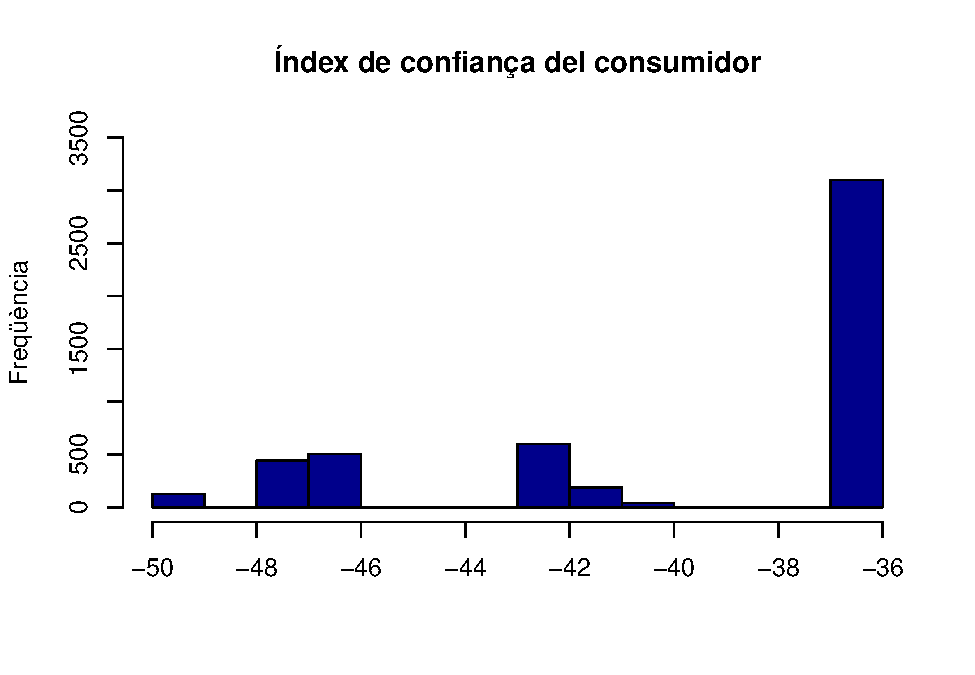
\includegraphics{Entrega-1_files/figure-latex/unnamed-chunk-27-1.pdf}

\hypertarget{euribor-3-month-rate}{%
\paragraph{Euribor 3 month rate}\label{euribor-3-month-rate}}

\begin{Shaded}
\begin{Highlighting}[]
\FunctionTok{hist}\NormalTok{(df}\SpecialCharTok{$}\NormalTok{euribor3m,}
     \AttributeTok{ylim =} \FunctionTok{c}\NormalTok{(}\DecValTok{0}\NormalTok{, }\DecValTok{4000}\NormalTok{),}
        \AttributeTok{col =} \StringTok{"blue4"}\NormalTok{,}
        \AttributeTok{xlab =} \StringTok{""}\NormalTok{,}
        \AttributeTok{ylab =} \StringTok{"Freqüència"}\NormalTok{,}
        \AttributeTok{main =} \StringTok{"Índex euribor a 3 mesos"}\NormalTok{)}
\end{Highlighting}
\end{Shaded}

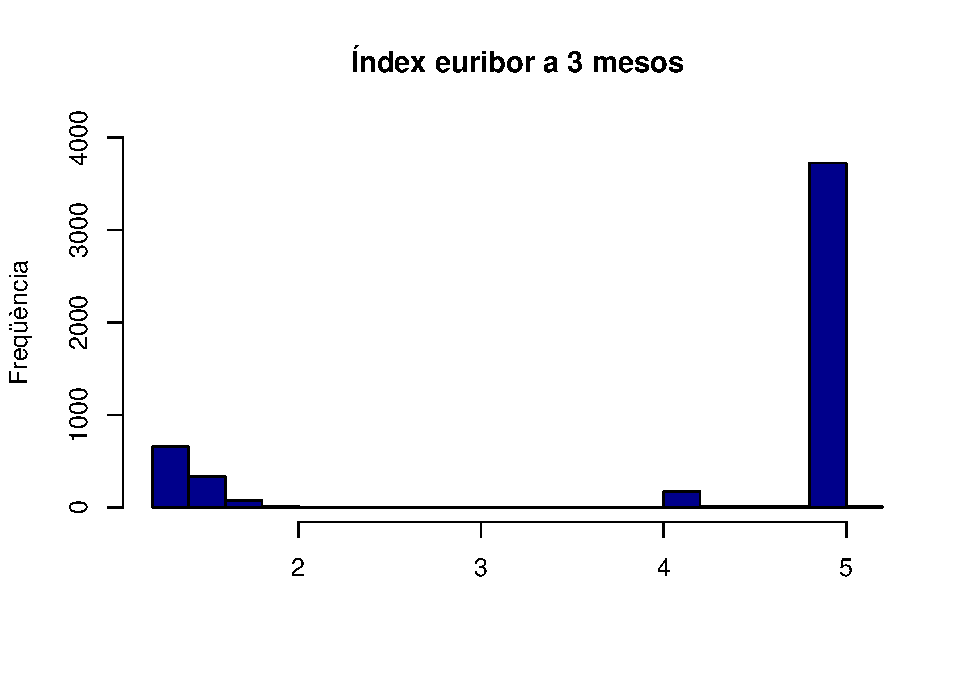
\includegraphics{Entrega-1_files/figure-latex/unnamed-chunk-28-1.pdf}

\hypertarget{number-of-employees}{%
\paragraph{Number of employees}\label{number-of-employees}}

\begin{Shaded}
\begin{Highlighting}[]
\FunctionTok{hist}\NormalTok{(df}\SpecialCharTok{$}\NormalTok{nr.employed,}
     \AttributeTok{ylim =} \FunctionTok{c}\NormalTok{(}\DecValTok{0}\NormalTok{, }\DecValTok{3500}\NormalTok{),}
        \AttributeTok{col =} \StringTok{"blue4"}\NormalTok{,}
        \AttributeTok{xlab =} \StringTok{""}\NormalTok{,}
        \AttributeTok{ylab =} \StringTok{"Freqüència"}\NormalTok{,}
        \AttributeTok{main =} \StringTok{"Nombre d\textquotesingle{}empleats"}\NormalTok{)}
\end{Highlighting}
\end{Shaded}

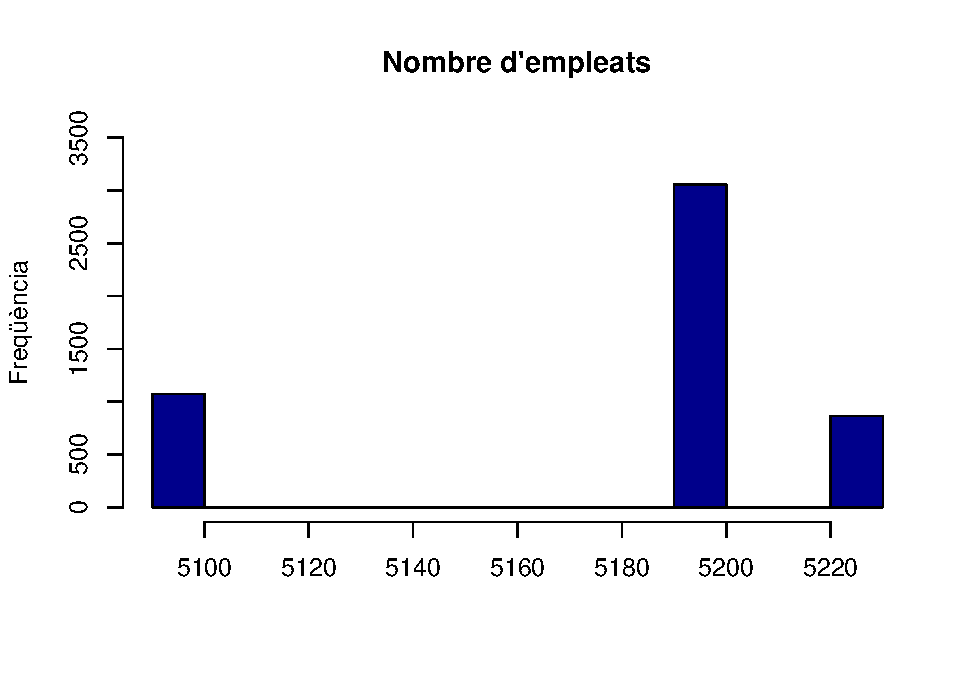
\includegraphics{Entrega-1_files/figure-latex/unnamed-chunk-29-1.pdf}

\hypertarget{subscribed-deposit}{%
\paragraph{Subscribed deposit}\label{subscribed-deposit}}

\begin{Shaded}
\begin{Highlighting}[]
\FunctionTok{pie}\NormalTok{(}\FunctionTok{prop.table}\NormalTok{(}\FunctionTok{table}\NormalTok{(df}\SpecialCharTok{$}\NormalTok{y)),}
        \AttributeTok{col =} \FunctionTok{c}\NormalTok{(}\StringTok{"brown3"}\NormalTok{, }\StringTok{"green3"}\NormalTok{),}
        \AttributeTok{main =} \StringTok{"Distribució de la variable y"}\NormalTok{)}
\end{Highlighting}
\end{Shaded}

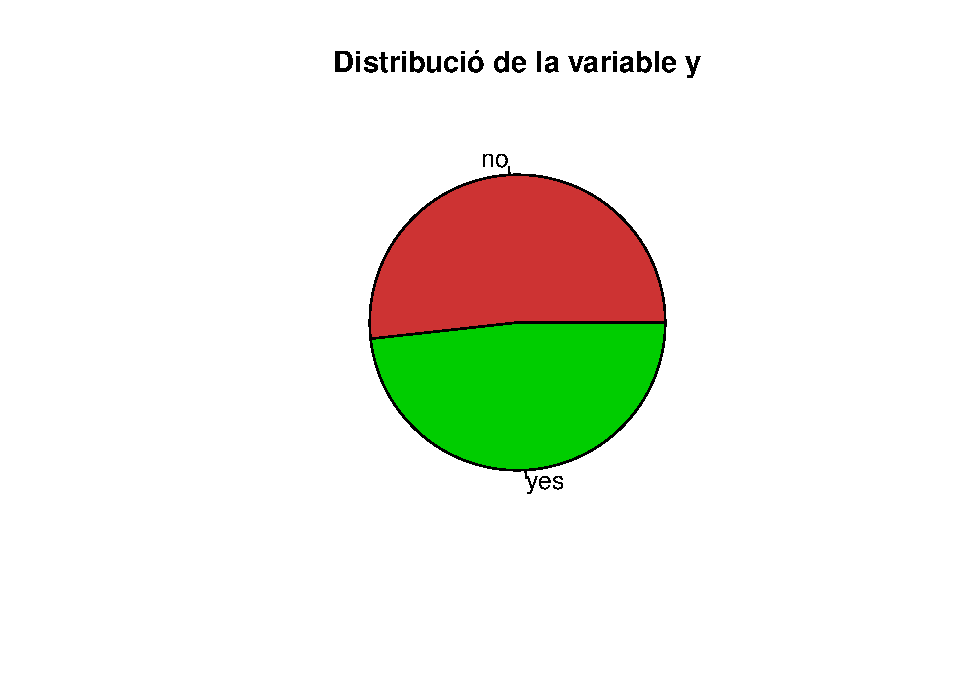
\includegraphics{Entrega-1_files/figure-latex/unnamed-chunk-30-1.pdf}

\hypertarget{qualitat-de-les-dades}{%
\subsection{Qualitat de les dades}\label{qualitat-de-les-dades}}

\hypertarget{per-variable}{%
\subsubsection{Per variable}\label{per-variable}}

\hypertarget{nombre-de-missings}{%
\paragraph{Nombre de missings}\label{nombre-de-missings}}

Passem tots els valors ``unknown'' a NA's per tractar-los com a missings
i contem el total de NA's per variable.

\begin{Shaded}
\begin{Highlighting}[]
\NormalTok{df[df }\SpecialCharTok{==} \StringTok{"unknown"}\NormalTok{] }\OtherTok{\textless{}{-}} \ConstantTok{NA}

\CommentTok{\#Mostrem el nombre de missings per variable}
\FunctionTok{colSums}\NormalTok{(}\FunctionTok{is.na}\NormalTok{(df))}
\end{Highlighting}
\end{Shaded}

\begin{verbatim}
##            age            job        marital      education        default 
##              0             54             10            239           1244 
##        housing           loan        contact          month    day_of_week 
##            133            133              0              0              0 
##       duration       campaign          pdays       previous       poutcome 
##              0              0              0              0              0 
##   emp.var.rate cons.price.idx  cons.conf.idx      euribor3m    nr.employed 
##              0              0              0              0              0 
##              y        age_num 
##              0              0
\end{verbatim}

\hypertarget{nombre-derrors}{%
\paragraph{Nombre d'errors}\label{nombre-derrors}}

1- Que una persona tingui pdays de 999 i que previous ``yes'' és una
contradicció

\begin{Shaded}
\begin{Highlighting}[]
\NormalTok{err\_ind }\OtherTok{\textless{}{-}} \FunctionTok{which}\NormalTok{(df}\SpecialCharTok{$}\NormalTok{pdays }\SpecialCharTok{==} \DecValTok{999} \SpecialCharTok{\&}\NormalTok{ df}\SpecialCharTok{$}\NormalTok{previous }\SpecialCharTok{==} \StringTok{"Yes"}\NormalTok{)}
\FunctionTok{length}\NormalTok{(err\_ind)}
\end{Highlighting}
\end{Shaded}

\begin{verbatim}
## [1] 193
\end{verbatim}

\begin{Shaded}
\begin{Highlighting}[]
\NormalTok{df}\SpecialCharTok{$}\NormalTok{previous[err\_ind]}\OtherTok{\textless{}{-}}\ConstantTok{NA}
\NormalTok{df}\SpecialCharTok{$}\NormalTok{pdays[err\_ind]}\OtherTok{\textless{}{-}}\ConstantTok{NA}
\end{Highlighting}
\end{Shaded}

\hypertarget{nombre-doutliers}{%
\paragraph{Nombre d'outliers}\label{nombre-doutliers}}

Busquem els outliers de les variables utilitzant la tècnica del tercer
quantil

\begin{Shaded}
\begin{Highlighting}[]
\FunctionTok{boxplot}\NormalTok{(df}\SpecialCharTok{$}\NormalTok{duration, }\AttributeTok{col =} \StringTok{"blue4"}\NormalTok{)}
\NormalTok{treshold }\OtherTok{\textless{}{-}} \FunctionTok{quantile}\NormalTok{(df}\SpecialCharTok{$}\NormalTok{duration, }\FloatTok{0.75}\NormalTok{)}\SpecialCharTok{*}\DecValTok{3}
\FunctionTok{abline}\NormalTok{(}\AttributeTok{h =}\NormalTok{ treshold, }\AttributeTok{col =} \StringTok{"red"}\NormalTok{, }\AttributeTok{lty =} \StringTok{"dashed"}\NormalTok{)}
\end{Highlighting}
\end{Shaded}

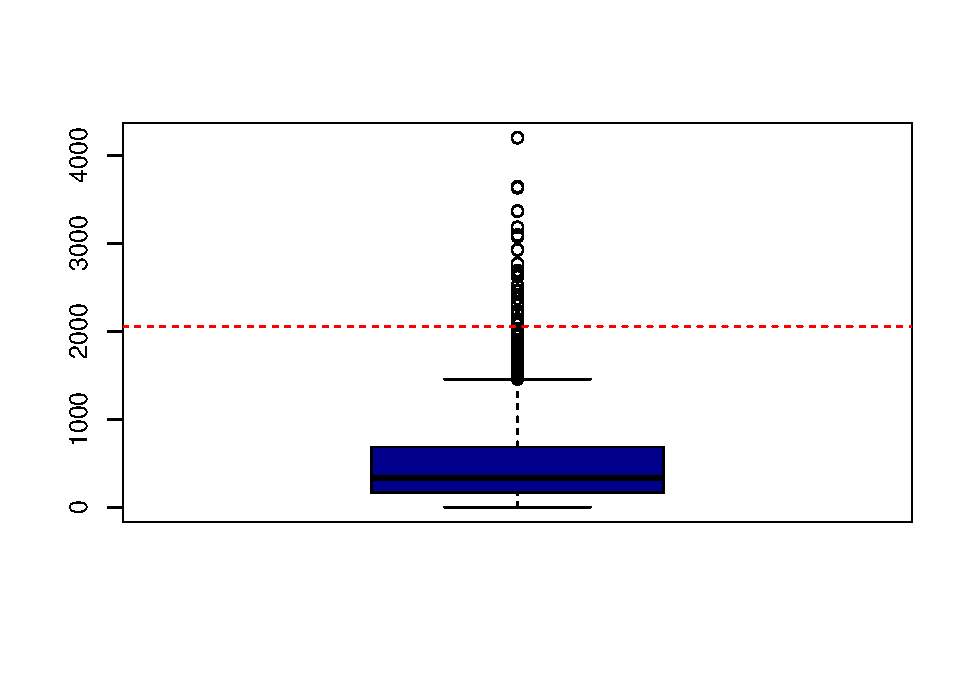
\includegraphics{Entrega-1_files/figure-latex/unnamed-chunk-33-1.pdf}

Trobem el nombre d'outliers

\begin{Shaded}
\begin{Highlighting}[]
\NormalTok{out\_dur }\OtherTok{\textless{}{-}} \FunctionTok{which}\NormalTok{(df}\SpecialCharTok{$}\NormalTok{duration }\SpecialCharTok{\textgreater{}}\NormalTok{ treshold)}
\FunctionTok{length}\NormalTok{(out\_dur)}
\end{Highlighting}
\end{Shaded}

\begin{verbatim}
## [1] 30
\end{verbatim}

\begin{Shaded}
\begin{Highlighting}[]
\FunctionTok{boxplot}\NormalTok{(df}\SpecialCharTok{$}\NormalTok{campaign, }\AttributeTok{col =} \StringTok{"blue4"}\NormalTok{)}
\NormalTok{treshold }\OtherTok{\textless{}{-}} \FunctionTok{quantile}\NormalTok{(df}\SpecialCharTok{$}\NormalTok{campaign, }\FloatTok{0.75}\NormalTok{)}\SpecialCharTok{*}\DecValTok{3}
\FunctionTok{abline}\NormalTok{(}\AttributeTok{h =}\NormalTok{ treshold, }\AttributeTok{col =} \StringTok{"red"}\NormalTok{, }\AttributeTok{lty =} \StringTok{"dashed"}\NormalTok{)}
\end{Highlighting}
\end{Shaded}

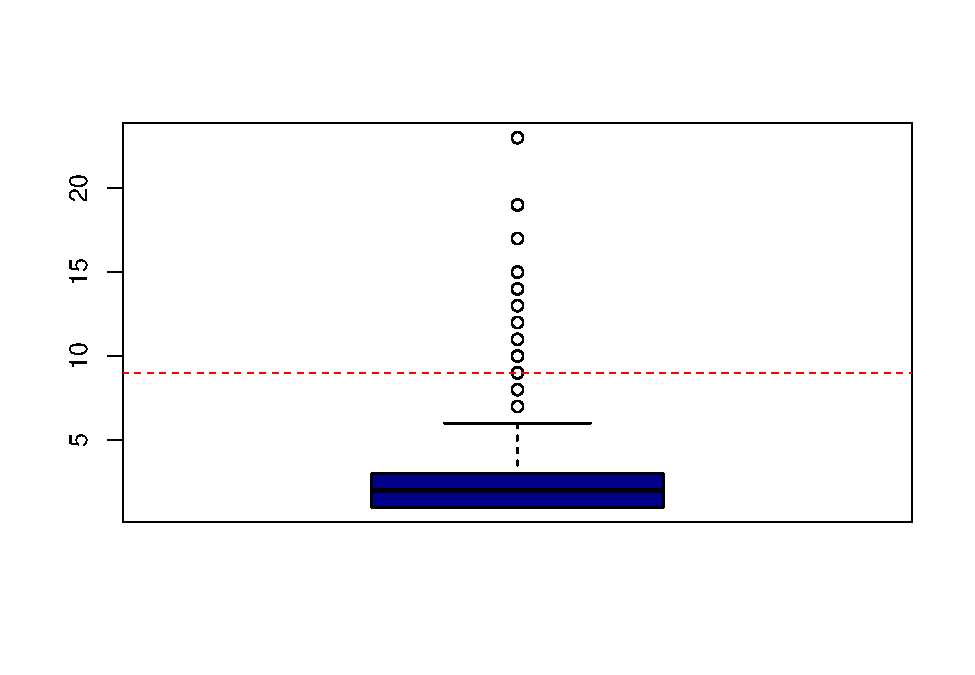
\includegraphics{Entrega-1_files/figure-latex/unnamed-chunk-35-1.pdf}

Trobem el nombre d'outliers

\begin{Shaded}
\begin{Highlighting}[]
\NormalTok{out\_camp }\OtherTok{\textless{}{-}} \FunctionTok{which}\NormalTok{(df}\SpecialCharTok{$}\NormalTok{campaign }\SpecialCharTok{\textgreater{}}\NormalTok{ treshold)}
\FunctionTok{length}\NormalTok{(out\_camp)}
\end{Highlighting}
\end{Shaded}

\begin{verbatim}
## [1] 45
\end{verbatim}

\hypertarget{ranking-de-variables-amb-muxe9s-valors-na}{%
\paragraph{Ranking de variables amb més valors
NA}\label{ranking-de-variables-amb-muxe9s-valors-na}}

\begin{Shaded}
\begin{Highlighting}[]
\NormalTok{nas\_per\_var }\OtherTok{\textless{}{-}} \FunctionTok{data.frame}\NormalTok{(}\AttributeTok{num\_nas =} \FunctionTok{colSums}\NormalTok{(}\FunctionTok{is.na}\NormalTok{(df)),}
                          \AttributeTok{variable =} \FunctionTok{names}\NormalTok{(df))}

\CommentTok{\# Ordenem el data frame per nombre de NA\textquotesingle{}s descendent}
\NormalTok{nas\_per\_var }\OtherTok{\textless{}{-}}\NormalTok{ nas\_per\_var[}\FunctionTok{order}\NormalTok{(}\SpecialCharTok{{-}}\NormalTok{nas\_per\_var}\SpecialCharTok{$}\NormalTok{num\_nas),]}

\CommentTok{\# Fem el gràfic de barres}
\FunctionTok{barplot}\NormalTok{(nas\_per\_var}\SpecialCharTok{$}\NormalTok{num\_nas,}
        \AttributeTok{names.arg =}\NormalTok{ nas\_per\_var}\SpecialCharTok{$}\NormalTok{variable,}
        \AttributeTok{ylim =} \FunctionTok{c}\NormalTok{(}\DecValTok{0}\NormalTok{, }\DecValTok{1400}\NormalTok{),}
        \AttributeTok{col =} \StringTok{"blue4"}\NormalTok{,}
        \AttributeTok{ylab =} \StringTok{"Nombre de NA\textquotesingle{}s"}\NormalTok{,}
        \AttributeTok{main =} \StringTok{"Ranking de variables amb més NA\textquotesingle{}s"}\NormalTok{,}
        \AttributeTok{las =} \DecValTok{2}\NormalTok{)}
\end{Highlighting}
\end{Shaded}

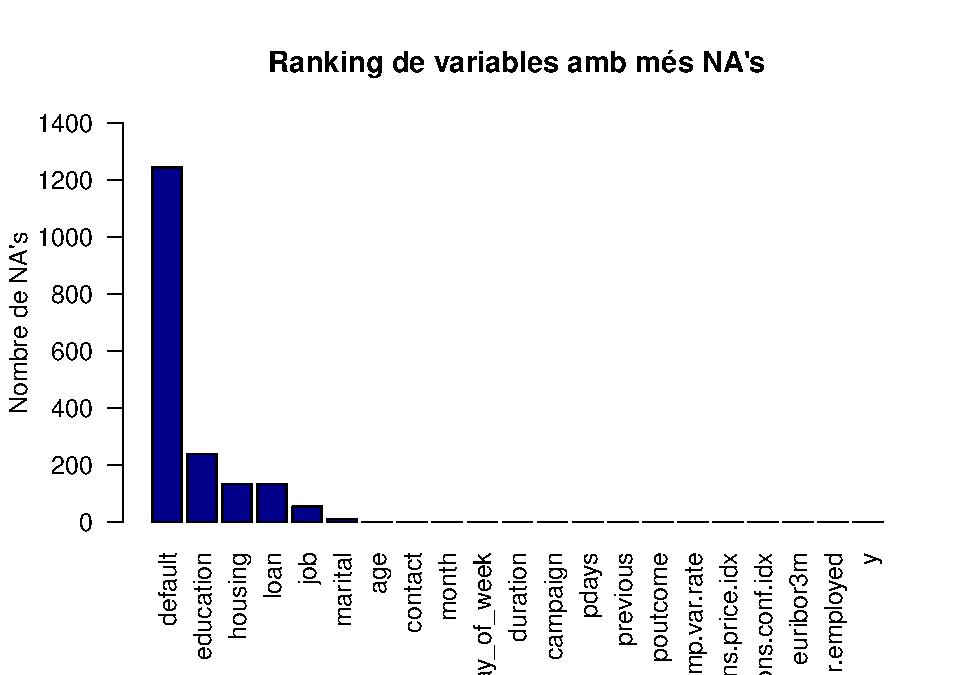
\includegraphics{Entrega-1_files/figure-latex/unnamed-chunk-37-1.pdf}

\hypertarget{per-individus}{%
\subsubsection{Per individus}\label{per-individus}}

Tornem a recuperar els valors de pdays i previous per no contar-los com
a missings, sino com a errors.

\begin{Shaded}
\begin{Highlighting}[]
\NormalTok{df}\SpecialCharTok{$}\NormalTok{pdays[err\_ind]}\OtherTok{\textless{}{-}}\DecValTok{999}
\NormalTok{df}\SpecialCharTok{$}\NormalTok{previous[err\_ind]}\OtherTok{\textless{}{-}}\StringTok{"Yes"}
\end{Highlighting}
\end{Shaded}

\hypertarget{nombre-de-missings-1}{%
\paragraph{Nombre de missings}\label{nombre-de-missings-1}}

\begin{Shaded}
\begin{Highlighting}[]
\NormalTok{n\_missings }\OtherTok{\textless{}{-}} \FunctionTok{rowSums}\NormalTok{(}\FunctionTok{is.na}\NormalTok{(df))}
\FunctionTok{table}\NormalTok{(n\_missings)}
\end{Highlighting}
\end{Shaded}

\begin{verbatim}
## n_missings
##    0    1    2    3    4 
## 3506 1250  174   65    5
\end{verbatim}

\hypertarget{nombre-derrors-1}{%
\paragraph{Nombre d'errors}\label{nombre-derrors-1}}

Com que només hem detectat un error, que pdays sigui 999 i previous
sigui ``yes'', sabem que tenim 193 combinacions de valors que compleixen
l'error. Per tant, tindrem que 193 individus tenen 2 errors (1 a pdays i
1 a previous) i la resta (4807) no tenen cap error.

Esborrarem la variable pdays ja que no ens aporta cap informació
adicional.

\begin{Shaded}
\begin{Highlighting}[]
\NormalTok{df }\OtherTok{\textless{}{-}} \FunctionTok{subset}\NormalTok{(df, }\AttributeTok{select =} \SpecialCharTok{{-}}\NormalTok{pdays)}
\end{Highlighting}
\end{Shaded}

\hypertarget{nombre-doutliers-1}{%
\paragraph{Nombre d'outliers}\label{nombre-doutliers-1}}

\begin{Shaded}
\begin{Highlighting}[]
\NormalTok{out\_ind }\OtherTok{\textless{}{-}} \FunctionTok{rowSums}\NormalTok{(}\FunctionTok{cbind}\NormalTok{(}\FunctionTok{as.numeric}\NormalTok{(df}\SpecialCharTok{$}\NormalTok{duration }\SpecialCharTok{\%in\%}\NormalTok{ out\_dur), }\FunctionTok{as.numeric}\NormalTok{(df}\SpecialCharTok{$}\NormalTok{campaign }\SpecialCharTok{\%in\%}\NormalTok{ out\_camp)))}
\FunctionTok{table}\NormalTok{(out\_ind)}
\end{Highlighting}
\end{Shaded}

\begin{verbatim}
## out_ind
##    0    1 
## 4934   66
\end{verbatim}

\hypertarget{afegim-variable-que-conta-els-na}{%
\paragraph{Afegim variable que conta els
NA}\label{afegim-variable-que-conta-els-na}}

Abans de contar els missings, passarem a NA's els index de les variables
que hem trobat errors o outliers.

\begin{Shaded}
\begin{Highlighting}[]
\NormalTok{df}\SpecialCharTok{$}\NormalTok{campaign[out\_camp]}\OtherTok{\textless{}{-}}\ConstantTok{NA}
\NormalTok{df}\SpecialCharTok{$}\NormalTok{duration[out\_dur]}\OtherTok{\textless{}{-}}\ConstantTok{NA}
\NormalTok{df}\SpecialCharTok{$}\NormalTok{previous[err\_ind]}\OtherTok{\textless{}{-}}\ConstantTok{NA}
\end{Highlighting}
\end{Shaded}

Creem la nova variable i contem els NA's

\begin{Shaded}
\begin{Highlighting}[]
\NormalTok{df}\SpecialCharTok{$}\NormalTok{na\_count }\OtherTok{\textless{}{-}} \FunctionTok{apply}\NormalTok{(df, }\DecValTok{1}\NormalTok{, }\ControlFlowTok{function}\NormalTok{(x) }\FunctionTok{sum}\NormalTok{(}\FunctionTok{is.na}\NormalTok{(x)))}
\end{Highlighting}
\end{Shaded}

\hypertarget{relaciuxf3-entre-grup-dedat-i-valors-atuxedpics}{%
\paragraph{Relació entre grup d'edat i valors
atípics}\label{relaciuxf3-entre-grup-dedat-i-valors-atuxedpics}}

Respecte els grups d'edat que hem definit anteriorment, volem veure quin
d'aquests grups és més propenç a tenir missings (dins dels missings hi
ha outliers i errors).

\begin{Shaded}
\begin{Highlighting}[]
\NormalTok{missings\_edat }\OtherTok{\textless{}{-}} \FunctionTok{aggregate}\NormalTok{(df}\SpecialCharTok{$}\NormalTok{na\_count, }\AttributeTok{by =} \FunctionTok{list}\NormalTok{(df}\SpecialCharTok{$}\NormalTok{age), sum)}
\NormalTok{missings\_edat }\OtherTok{\textless{}{-}}\NormalTok{ missings\_edat[}\FunctionTok{order}\NormalTok{(missings\_edat}\SpecialCharTok{$}\NormalTok{x, }\AttributeTok{decreasing =} \ConstantTok{TRUE}\NormalTok{), ]}
\FunctionTok{names}\NormalTok{(missings\_edat) }\OtherTok{\textless{}{-}} \FunctionTok{c}\NormalTok{(}\StringTok{"Grup d\textquotesingle{}edat"}\NormalTok{, }\StringTok{"Missings"}\NormalTok{)}
\NormalTok{missings\_edat}
\end{Highlighting}
\end{Shaded}

\begin{verbatim}
##   Grup d'edat Missings
## 2  Jove-Adult     1257
## 3       Adult      758
## 1        Jove       53
## 4        Gran       13
\end{verbatim}

\hypertarget{imputaciuxf3-de-missings}{%
\subsubsection{Imputació de missings}\label{imputaciuxf3-de-missings}}

\hypertarget{variables-categuxf2riques}{%
\paragraph{Variables categòriques}\label{variables-categuxf2riques}}

Imputem tots els NAs que tenim en el conjunt de variables categòriques
(var\_cat).

Dades abans de imputar.

\begin{Shaded}
\begin{Highlighting}[]
\NormalTok{var\_cat }\OtherTok{\textless{}{-}} \FunctionTok{c}\NormalTok{(}\StringTok{"age"}\NormalTok{, }\StringTok{"job"}\NormalTok{, }\StringTok{"marital"}\NormalTok{, }\StringTok{"education"}\NormalTok{, }\StringTok{"housing"}\NormalTok{, }\StringTok{"loan"}\NormalTok{, }\StringTok{"contact"}\NormalTok{, }\StringTok{"month"}\NormalTok{, }\StringTok{"day\_of\_week"}\NormalTok{, }\StringTok{"previous"}\NormalTok{, }\StringTok{"poutcome"}\NormalTok{, }\StringTok{"y"}\NormalTok{) }\CommentTok{\#Obviarem la variable "default" ja que té masses missings per imputar}
\FunctionTok{summary}\NormalTok{(df[,var\_cat])}
\end{Highlighting}
\end{Shaded}

\begin{verbatim}
##          age                job           marital    
##  Jove      : 172   blue-collar:1251   divorced: 537  
##  Jove-Adult:3413   admin.     :1158   married :3148  
##  Adult     :1375   technician : 755   single  :1305  
##  Gran      :  40   services   : 529   unknown :   0  
##                    unemployed : 522   NA's    :  10  
##                    (Other)    : 731                  
##                    NA's       :  54                  
##                education       housing          loan           contact    
##  basic              :1664   no     :2400   no     :4150   cellular :1825  
##  high.school        :1170   unknown:   0   unknown:   0   telephone:3175  
##  illiterate         :   2   yes    :2467   yes    : 717                   
##  professional.course: 603   NA's   : 133   NA's   : 133                   
##  university.degree  :1322                                                 
##  unknown            :   0                                                 
##  NA's               : 239                                                 
##      month      day_of_week previous           poutcome      y       
##  may    :3333   mon:1075    No  :4719   failure    : 197   no :2588  
##  apr    : 442   tue:1211    Yes :  88   nonexistent:4719   yes:2412  
##  jul    : 407   wed: 881    NA's: 193   success    :  84             
##  aug    : 271   thu: 993                                             
##  nov    : 190   fri: 840                                             
##  jun    : 188   sat:   0                                             
##  (Other): 169   sun:   0
\end{verbatim}

\begin{Shaded}
\begin{Highlighting}[]
\NormalTok{res.immca}\OtherTok{\textless{}{-}}\FunctionTok{imputeMCA}\NormalTok{(df[,var\_cat],}\AttributeTok{ncp =} \FunctionTok{length}\NormalTok{(var\_cat)}\SpecialCharTok{{-}}\DecValTok{1}\NormalTok{)}
\FunctionTok{summary}\NormalTok{(res.immca}\SpecialCharTok{$}\NormalTok{completeObs)}
\end{Highlighting}
\end{Shaded}

\begin{verbatim}
##          age                  job           marital    
##  Jove      : 172   admin.       :1169   divorced: 537  
##  Jove-Adult:3413   blue-collar  :1292   married :3158  
##  Adult     :1375   management   : 379   single  :1305  
##  Gran      :  40   self-employed: 352                  
##                    services     : 530                  
##                    technician   : 756                  
##                    unemployed   : 522                  
##                education    housing     loan           contact    
##  basic              :1767   no :2473   no :4283   cellular :1825  
##  high.school        :1212   yes:2527   yes: 717   telephone:3175  
##  illiterate         :   2                                         
##  professional.course: 632                                         
##  university.degree  :1387                                         
##                                                                   
##                                                                   
##      month      day_of_week previous          poutcome      y       
##  may    :3333   mon:1075    No :4912   failure    : 197   no :2588  
##  apr    : 442   tue:1211    Yes:  88   nonexistent:4719   yes:2412  
##  jul    : 407   wed: 881               success    :  84             
##  aug    : 271   thu: 993                                            
##  nov    : 190   fri: 840                                            
##  jun    : 188                                                       
##  (Other): 169
\end{verbatim}

\begin{Shaded}
\begin{Highlighting}[]
\NormalTok{df[,var\_cat]}\OtherTok{\textless{}{-}}\NormalTok{res.immca}\SpecialCharTok{$}\NormalTok{completeObs}
\end{Highlighting}
\end{Shaded}

\hypertarget{variables-numuxe8riques}{%
\paragraph{Variables numèriques}\label{variables-numuxe8riques}}

Imputem tots els NAs que tenim en el conjunt de variables numeriques
(var\_num).

Dades abans de imputar.

\begin{Shaded}
\begin{Highlighting}[]
\NormalTok{var\_num }\OtherTok{\textless{}{-}} \FunctionTok{c}\NormalTok{(}\StringTok{"duration"}\NormalTok{, }\StringTok{"campaign"}\NormalTok{, }\StringTok{"emp.var.rate"}\NormalTok{, }\StringTok{"cons.conf.idx"}\NormalTok{, }\StringTok{"cons.price.idx"}\NormalTok{, }\StringTok{"euribor3m"}\NormalTok{, }\StringTok{"nr.employed"}\NormalTok{)}
\FunctionTok{summary}\NormalTok{(df[,var\_num])}
\end{Highlighting}
\end{Shaded}

\begin{verbatim}
##     duration         campaign      emp.var.rate     cons.conf.idx   
##  Min.   :   3.0   Min.   :1.000   Min.   :-1.8000   Min.   :-50.00  
##  1st Qu.: 170.0   1st Qu.:1.000   1st Qu.:-0.1000   1st Qu.:-42.70  
##  Median : 334.0   Median :2.000   Median : 1.1000   Median :-36.40  
##  Mean   : 463.6   Mean   :2.065   Mean   : 0.4737   Mean   :-39.63  
##  3rd Qu.: 676.8   3rd Qu.:3.000   3rd Qu.: 1.1000   3rd Qu.:-36.40  
##  Max.   :2033.0   Max.   :9.000   Max.   : 1.4000   Max.   :-36.10  
##  NA's   :30       NA's   :45                                        
##  cons.price.idx    euribor3m      nr.employed  
##  Min.   :92.76   Min.   :1.244   Min.   :5099  
##  1st Qu.:93.20   1st Qu.:4.343   1st Qu.:5191  
##  Median :93.99   Median :4.856   Median :5191  
##  Mean   :93.72   Mean   :4.100   Mean   :5178  
##  3rd Qu.:93.99   3rd Qu.:4.857   3rd Qu.:5191  
##  Max.   :94.47   Max.   :5.045   Max.   :5228  
## 
\end{verbatim}

Imputació dels missings.

\begin{Shaded}
\begin{Highlighting}[]
\NormalTok{res.impca}\OtherTok{\textless{}{-}}\FunctionTok{imputePCA}\NormalTok{(df[,var\_num],}\AttributeTok{ncp =} \FunctionTok{length}\NormalTok{(var\_num)}\SpecialCharTok{{-}}\DecValTok{1}\NormalTok{)}
\FunctionTok{summary}\NormalTok{(res.impca}\SpecialCharTok{$}\NormalTok{completeObs)}
\end{Highlighting}
\end{Shaded}

\begin{verbatim}
##     duration         campaign      emp.var.rate     cons.conf.idx   
##  Min.   :   3.0   Min.   :1.000   Min.   :-1.8000   Min.   :-50.00  
##  1st Qu.: 171.0   1st Qu.:1.000   1st Qu.:-0.1000   1st Qu.:-42.70  
##  Median : 336.0   Median :2.000   Median : 1.1000   Median :-36.40  
##  Mean   : 464.8   Mean   :2.068   Mean   : 0.4737   Mean   :-39.63  
##  3rd Qu.: 680.0   3rd Qu.:3.000   3rd Qu.: 1.1000   3rd Qu.:-36.40  
##  Max.   :2033.0   Max.   :9.000   Max.   : 1.4000   Max.   :-36.10  
##  cons.price.idx    euribor3m      nr.employed  
##  Min.   :92.76   Min.   :1.244   Min.   :5099  
##  1st Qu.:93.20   1st Qu.:4.343   1st Qu.:5191  
##  Median :93.99   Median :4.856   Median :5191  
##  Mean   :93.72   Mean   :4.100   Mean   :5178  
##  3rd Qu.:93.99   3rd Qu.:4.857   3rd Qu.:5191  
##  Max.   :94.47   Max.   :5.045   Max.   :5228
\end{verbatim}

\begin{Shaded}
\begin{Highlighting}[]
\NormalTok{df[,var\_num ]}\OtherTok{\textless{}{-}}\NormalTok{res.impca}\SpecialCharTok{$}\NormalTok{completeObs}
\end{Highlighting}
\end{Shaded}

\hypertarget{profiling}{%
\subsection{Profiling}\label{profiling}}

\hypertarget{variables-categuxf2riques-1}{%
\subsubsection{Variables
categòriques}\label{variables-categuxf2riques-1}}

\begin{Shaded}
\begin{Highlighting}[]
\CommentTok{\#edat}
\NormalTok{res.catdes}\OtherTok{\textless{}{-}}\FunctionTok{catdes}\NormalTok{(df,}\FunctionTok{grep}\NormalTok{(}\StringTok{"\^{}y$"}\NormalTok{, }\FunctionTok{colnames}\NormalTok{(df)), }\AttributeTok{proba=}\FloatTok{0.05}\NormalTok{)}
\NormalTok{res.catdes}\SpecialCharTok{$}\NormalTok{test.chi2 }\CommentTok{\# relació entre les variables y la variable resposta}
\end{Highlighting}
\end{Shaded}

\begin{verbatim}
##                  p.value df
## contact     0.000000e+00  1
## month       0.000000e+00  8
## poutcome    4.272175e-70  2
## default     1.928184e-43  1
## day_of_week 3.199213e-31  4
## marital     1.423436e-23  2
## previous    1.085202e-22  1
## age         2.484262e-22  3
## education   3.990582e-22  4
## job         4.547525e-15  6
## housing     7.595941e-11  1
\end{verbatim}

\begin{Shaded}
\begin{Highlighting}[]
\NormalTok{res.catdes}\SpecialCharTok{$}\NormalTok{category }
\end{Highlighting}
\end{Shaded}

\begin{verbatim}
## $no
##                              Cla/Mod    Mod/Cla Global       p.value     v.test
## month=may                   77.64776 100.000000  66.66  0.000000e+00        Inf
## contact=telephone           81.51181 100.000000  63.50  0.000000e+00        Inf
## poutcome=nonexistent        54.84213 100.000000  94.38  1.396630e-93  20.521050
## default=NA                  68.72990  33.037094  24.88  2.743947e-44  13.959750
## previous=No                 52.68730 100.000000  98.24  5.977949e-29  11.166052
## day_of_week=tue             64.07927  29.984544  24.22  3.778666e-23   9.909677
## marital=married             56.71311  69.204019  63.16  4.208146e-20   9.182598
## education=basic             59.59253  40.687790  35.34  2.212776e-16   8.209952
## job=blue-collar             59.98452  29.945904  25.84  5.702943e-12   6.886880
## housing=no                  56.40922  53.902628  49.46  7.492004e-11   6.510462
## age=Adult                   57.67273  30.641422  27.50  2.478903e-07   5.159288
## day_of_week=mon             56.74419  23.570325  21.50  2.206025e-04   3.694174
## job=services                58.49057  11.978362  10.60  1.022175e-03   3.284351
## job=unemployed              46.55172   9.389490  10.44  1.196767e-02  -2.513096
## job=technician              47.08995  13.755796  15.12  5.330588e-03  -2.786346
## day_of_week=fri             47.14286  15.301391  16.80  3.355222e-03  -2.933168
## job=admin.                  45.16681  20.401855  23.38  2.586795e-07  -5.151305
## day_of_week=wed             43.47333  14.799073  17.62  5.911229e-08  -5.421466
## day_of_week=thu             42.59819  16.344668  19.86  1.088140e-10  -6.454169
## housing=yes                 47.21013  46.097372  50.54  7.492004e-11  -6.510462
## age=Jove                    27.32558   1.816074   3.44  4.108495e-11  -6.600111
## age=Gran                     0.00000   0.000000   0.80  1.832334e-13  -7.360492
## month=oct                    0.00000   0.000000   0.84  4.189623e-14  -7.554968
## education=university.degree 41.31218  22.140649  27.74  4.843918e-20  -9.167439
## marital=single              39.84674  20.092736  26.10  1.101467e-23 -10.032102
## poutcome=success             0.00000   0.000000   1.68  1.190303e-27 -10.897069
## previous=Yes                 0.00000   0.000000   1.76  5.977949e-29 -11.166052
## month=mar                    0.00000   0.000000   2.52  2.269537e-41 -13.472530
## default=no                  46.13951  66.962906  75.12  2.743947e-44 -13.959750
## month=jun                    0.00000   0.000000   3.76  5.976573e-62 -16.609220
## month=nov                    0.00000   0.000000   3.80  1.276337e-62 -16.701583
## poutcome=failure             0.00000   0.000000   3.94  5.700944e-65 -17.021382
## month=aug                    0.00000   0.000000   5.42  3.904937e-90 -20.131561
## month=jul                    0.00000   0.000000   8.14 5.437191e-138 -25.004681
## month=apr                    0.00000   0.000000   8.84 1.155522e-150 -26.143923
## contact=cellular             0.00000   0.000000  36.50  0.000000e+00       -Inf
## 
## $yes
##                               Cla/Mod   Mod/Cla Global       p.value     v.test
## contact=cellular            100.00000 75.663350  36.50  0.000000e+00        Inf
## month=apr                   100.00000 18.325041   8.84 1.155522e-150  26.143923
## month=jul                   100.00000 16.873964   8.14 5.437191e-138  25.004681
## month=aug                   100.00000 11.235489   5.42  3.904937e-90  20.131561
## poutcome=failure            100.00000  8.167496   3.94  5.700944e-65  17.021382
## month=nov                   100.00000  7.877280   3.80  1.276337e-62  16.701583
## month=jun                   100.00000  7.794362   3.76  5.976573e-62  16.609220
## default=no                   53.86049 83.872305  75.12  2.743947e-44  13.959750
## month=mar                   100.00000  5.223881   2.52  2.269537e-41  13.472530
## previous=Yes                100.00000  3.648425   1.76  5.977949e-29  11.166052
## poutcome=success            100.00000  3.482587   1.68  1.190303e-27  10.897069
## marital=single               60.15326 32.545605  26.10  1.101467e-23  10.032102
## education=university.degree  58.68782 33.747927  27.74  4.843918e-20   9.167439
## month=oct                   100.00000  1.741294   0.84  4.189623e-14   7.554968
## age=Gran                    100.00000  1.658375   0.80  1.832334e-13   7.360492
## age=Jove                     72.67442  5.182421   3.44  4.108495e-11   6.600111
## housing=yes                  52.78987 55.306799  50.54  7.492004e-11   6.510462
## day_of_week=thu              57.40181 23.631841  19.86  1.088140e-10   6.454169
## day_of_week=wed              56.52667 20.646766  17.62  5.911229e-08   5.421466
## job=admin.                   54.83319 26.575456  23.38  2.586795e-07   5.151305
## day_of_week=fri              52.85714 18.407960  16.80  3.355222e-03   2.933168
## job=technician               52.91005 16.583748  15.12  5.330588e-03   2.786346
## job=unemployed               53.44828 11.567164  10.44  1.196767e-02   2.513096
## job=services                 41.50943  9.121061  10.60  1.022175e-03  -3.284351
## day_of_week=mon              43.25581 19.278607  21.50  2.206025e-04  -3.694174
## age=Adult                    42.32727 24.129353  27.50  2.478903e-07  -5.159288
## housing=no                   43.59078 44.693201  49.46  7.492004e-11  -6.510462
## job=blue-collar              40.01548 21.434494  25.84  5.702943e-12  -6.886880
## education=basic              40.40747 29.601990  35.34  2.212776e-16  -8.209952
## marital=married              43.28689 56.674959  63.16  4.208146e-20  -9.182598
## day_of_week=tue              35.92073 18.034826  24.22  3.778666e-23  -9.909677
## previous=No                  47.31270 96.351575  98.24  5.977949e-29 -11.166052
## default=NA                   31.27010 16.127695  24.88  2.743947e-44 -13.959750
## poutcome=nonexistent         45.15787 88.349917  94.38  1.396630e-93 -20.521050
## month=may                    22.35224 30.887231  66.66  0.000000e+00       -Inf
## contact=telephone            18.48819 24.336650  63.50  0.000000e+00       -Inf
\end{verbatim}

\begin{Shaded}
\begin{Highlighting}[]
\NormalTok{res.catdes}\SpecialCharTok{$}\NormalTok{quanti  }\CommentTok{\# Global association to numeric variables}
\end{Highlighting}
\end{Shaded}

\begin{verbatim}
## $no
##                    v.test Mean in category Overall mean sd in category
## cons.conf.idx   53.169902      -36.4000000   -39.626300   0.000000e+00
## cons.price.idx  43.816029       93.9940000    93.722201   0.000000e+00
## euribor3m       38.675184        4.8560696     4.100294   8.352458e-04
## emp.var.rate    37.512348        1.1000000     0.473680   0.000000e+00
## nr.employed     22.081559     5191.0000000  5177.923760   0.000000e+00
## age_num          6.658336       41.0641422    40.159000   8.885746e+00
## na_count         6.469584        0.4741113     0.416200   6.947767e-01
## campaign        -3.462143        2.0011383     2.067662   1.294232e+00
## duration       -42.854275      243.9352241   464.790464   2.007280e+02
##                 Overall sd       p.value
## cons.conf.idx    4.4439989  0.000000e+00
## cons.price.idx   0.4543068  0.000000e+00
## euribor3m        1.4311845  0.000000e+00
## emp.var.rate     1.2228047 5.794591e-308
## nr.employed     43.3698783 4.754022e-108
## age_num          9.9560293  2.769453e-11
## na_count         0.6555742  9.827295e-11
## campaign         1.4072408  5.358914e-04
## duration       377.4405914  0.000000e+00
## 
## $yes
##                    v.test Mean in category Overall mean sd in category
## duration        42.854275      701.7611779   464.790464    378.9391840
## campaign         3.462143        2.1390405     2.067662      1.5159317
## na_count        -6.469584        0.3540630     0.416200      0.6045811
## age_num         -6.658336       39.1878109    40.159000     10.9058598
## nr.employed    -22.081559     5163.8933665  5177.923760     59.3196912
## emp.var.rate   -37.512348       -0.1983416     0.473680      1.4923455
## euribor3m      -38.675184        3.2893702     4.100294      1.7249824
## cons.price.idx -43.816029       93.4305701    93.722201      0.5133574
## cons.conf.idx  -53.169902      -43.0880182   -39.626300      4.2174971
##                 Overall sd       p.value
## duration       377.4405914  0.000000e+00
## campaign         1.4072408  5.358914e-04
## na_count         0.6555742  9.827295e-11
## age_num          9.9560293  2.769453e-11
## nr.employed     43.3698783 4.754022e-108
## emp.var.rate     1.2228047 5.794591e-308
## euribor3m        1.4311845  0.000000e+00
## cons.price.idx   0.4543068  0.000000e+00
## cons.conf.idx    4.4439989  0.000000e+00
\end{verbatim}

\begin{Shaded}
\begin{Highlighting}[]
\NormalTok{res.catdes}\SpecialCharTok{$}\NormalTok{quali }\CommentTok{\# Global association to factors}
\end{Highlighting}
\end{Shaded}

\begin{verbatim}
## NULL
\end{verbatim}

\textbf{Mes}: El mes en què es va realitzar l'última campanya de
màrqueting també sembla estar relacionat amb el resultat negatiu de la
variable target ``y''. En particular, els mesos de maig i juny tenen una
taxa de rebuig més alta que altres mesos, mentre que el març, septembre
i octubre estan molt relacionats amb un resultat positiu.

\textbf{Euribor3m}: El tipus d'interès a tres mesos (Euribor3m) és la
variable més fortament relacionada amb la variable target ``y'' segons
el nostre analisi i tractament de variables. Si l'Euribor3m és baix, és
més probable que el client contracti el dipòsit a termini. Si aquest és
alt, també és l'influenciador més gran en què el resultat acabi sent
negatiu.

\textbf{Poutcome}: La variable Poutcome (resultat de la campanya de
màrqueting anterior) també està fortament relacionada amb la variable
target ``y''. Si el resultat de la campanya anterior va ser exitós, és
més probable que el client contracti el dipòsit a termini.

\textbf{Duration}: També es veu altament relacionada amb el resultat.
Això pot ser degut a que com més temps duri la trucada, és més probable
que l'agent de vendes hagi tingut l'oportunitat de persuadir el client i
fer-li una oferta més atractiva.

\textbf{Job}: El tipus de treball del client també sembla estar
relacionat amb la variable target ``y''. Els estudiants i els jubilats
tenen més probabilitats de contractar el dipòsit a termini, mentre que
els treballadors autònoms i els desocupats tenen menys probabilitats.

\textbf{Contact}: La forma de contacte també està relacionada amb el
resultat de la variable target ``y''. Els clients contactats per telèfon
fix tenen més probabilitats de rebutjar el dipòsit a termini que aquells
contactats per correu electrònic o per telèfon mòbil.

\textbf{Age}: En general, els clients més joves tenen més probabilitats
de rebutjar el dipòsit a termini que els clients més grans.

\textbf{Campaign}: El nombre de contactes realitzats durant l'última
campanya de màrqueting també està relacionat amb el resultat negatiu de
la variable target ``y''. En general, com més contactes es realitzin, és
més probable que el client rebutgi el dipòsit a termini.

\hypertarget{variables-numuxe9riques}{%
\subsubsection{Variables numériques}\label{variables-numuxe9riques}}

\begin{Shaded}
\begin{Highlighting}[]
\CommentTok{\#duration}
\NormalTok{res.condes}\OtherTok{\textless{}{-}}\FunctionTok{condes}\NormalTok{(df,}\FunctionTok{grep}\NormalTok{(}\StringTok{"\^{}duration$"}\NormalTok{, }\FunctionTok{colnames}\NormalTok{(df)), }\AttributeTok{proba=}\FloatTok{0.05}\NormalTok{)}
\NormalTok{res.condes}\SpecialCharTok{$}\NormalTok{test.chi2 }\CommentTok{\# relació entre les variables y la variable resposta}
\end{Highlighting}
\end{Shaded}

\begin{verbatim}
## NULL
\end{verbatim}

\begin{Shaded}
\begin{Highlighting}[]
\NormalTok{res.condes}\SpecialCharTok{$}\NormalTok{category }
\end{Highlighting}
\end{Shaded}

\begin{verbatim}
##                               Estimate       p.value
## y=yes                        228.91298  0.000000e+00
## contact=cellular             165.16324 2.093855e-214
## month=jul                    333.85272 3.965288e-118
## month=aug                    280.72756  5.068452e-57
## month=jun                    341.05236  1.938499e-53
## month=nov                    208.13506  2.463898e-25
## poutcome=failure             106.55349  7.581864e-13
## day_of_week=wed               50.66271  1.397880e-06
## default=no                    21.12415  6.195630e-04
## marital=single                20.58647  2.151955e-03
## day_of_week=thu               26.20140  3.632670e-03
## housing=yes                   11.24417  3.517575e-02
## day_of_week=fri               19.96409  3.575222e-02
## age=Jove-Adult                57.19128  3.944233e-02
## housing=no                   -11.24417  3.517575e-02
## education=university.degree  -16.52057  1.044162e-02
## month=oct                   -245.16912  2.484858e-03
## marital=married              -19.32388  2.432148e-03
## day_of_week=mon              -36.34532  2.098132e-03
## job=unemployed               -47.45417  1.484963e-03
## age=Gran                    -146.97090  9.341034e-04
## default=NA                   -21.12415  6.195630e-04
## day_of_week=tue              -60.48287  3.926094e-09
## month=mar                   -265.09390  3.802976e-09
## poutcome=nonexistent         -90.99622  3.314190e-12
## month=may                   -178.18275 5.706054e-198
## contact=telephone           -165.16324 2.093855e-214
## y=no                        -228.91298  0.000000e+00
\end{verbatim}

\begin{Shaded}
\begin{Highlighting}[]
\NormalTok{res.condes}\SpecialCharTok{$}\NormalTok{quanti  }\CommentTok{\# Global association to numeric variables}
\end{Highlighting}
\end{Shaded}

\begin{verbatim}
##                correlation      p.value
## campaign        0.09357119 3.371081e-11
## nr.employed     0.05776931 4.364235e-05
## age_num        -0.05293015 1.808138e-04
## emp.var.rate   -0.08878741 3.193708e-10
## euribor3m      -0.12017447 1.509610e-17
## cons.price.idx -0.18889226 2.199788e-41
## cons.conf.idx  -0.29184702 9.343997e-99
\end{verbatim}

\begin{Shaded}
\begin{Highlighting}[]
\NormalTok{res.condes}\SpecialCharTok{$}\NormalTok{quali }\CommentTok{\# Global association to factors}
\end{Highlighting}
\end{Shaded}

\begin{verbatim}
##                       R2       p.value
## month       0.2687566917  0.000000e+00
## y           0.3673712587  0.000000e+00
## contact     0.1775236255 2.093855e-214
## day_of_week 0.0126405296  5.186401e-13
## poutcome    0.0108893480  1.316225e-12
## default     0.0023416784  6.195630e-04
## age         0.0027889411  2.967867e-03
## marital     0.0020923915  5.335796e-03
## housing     0.0008873747  3.517575e-02
## job         0.0026763395  3.729645e-02
\end{verbatim}

\textbf{y}: Hi ha una forta relació amb la variable categòrica y. En
particular, té sentit que una duració elevada de la trucada vingui de la
ma d'un resultat positiu, perquè l'agent de vendes va de poder explicar
i vendre el producte.

\textbf{Contacte}: La forma de contacte utilitzada en l'última campanya
de màrqueting té una alta correlació amb la durada de la trucada. En
particular, els clients contactats per telèfon mòbil tendeixen a tenir
una taxa més alta de contractació del servei/producte. Això implica una
relació creuada amb la duració com ja hem comentat.

\textbf{Previous}: La variable ``Previous'' representa el número de
contactes realitzats abans de l'última campanya de màrqueting. En
general, com més gran sigui el número de contactes, menor serà la durada
de l'última trucada. La relació entre ``Duration'' i ``Previous'' podria
explicar-se per la possibilitat que l'agent de vendes hagi hagut de
repetir informació prèviament proporcionada en trucades anteriors.

\hypertarget{identify-individuals-considered-as-multivariate-outliers}{%
\subsection{Identify individuals considered as multivariate
outliers}\label{identify-individuals-considered-as-multivariate-outliers}}

\begin{Shaded}
\begin{Highlighting}[]
\CommentTok{\# Perform multivariate outlier analysis using Moutlier function}
\NormalTok{outliers }\OtherTok{\textless{}{-}} \FunctionTok{Moutlier}\NormalTok{(df[, }\FunctionTok{c}\NormalTok{(}\StringTok{"age\_num"}\NormalTok{, }\StringTok{"duration"}\NormalTok{)], }\AttributeTok{quantile=} \FloatTok{0.995}\NormalTok{)}
\end{Highlighting}
\end{Shaded}

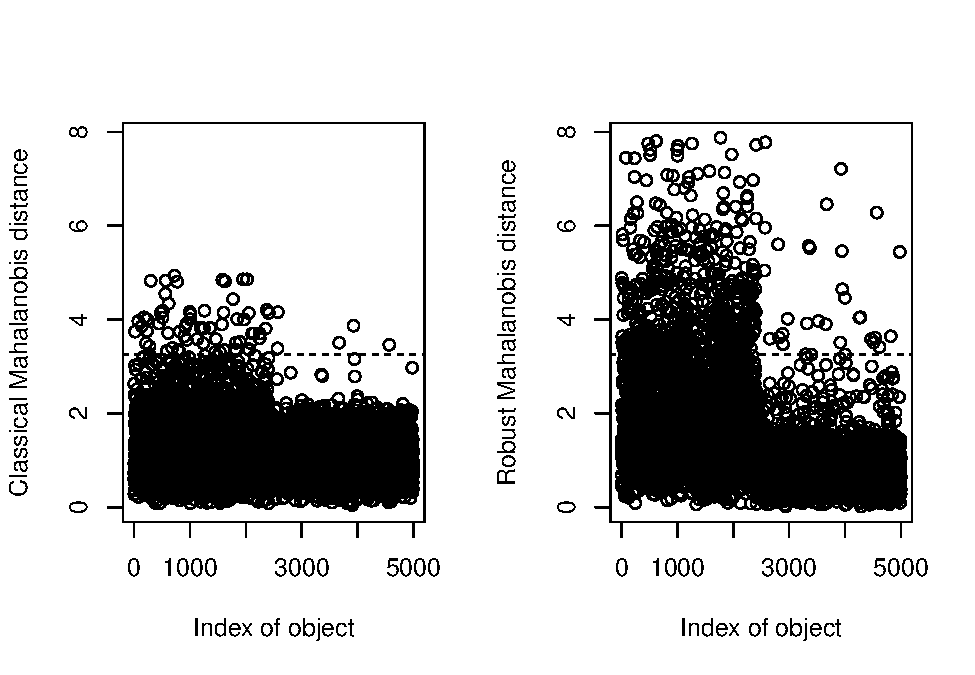
\includegraphics{Entrega-1_files/figure-latex/unnamed-chunk-51-1.pdf}

\begin{Shaded}
\begin{Highlighting}[]
\NormalTok{top5 }\OtherTok{\textless{}{-}} \FunctionTok{order}\NormalTok{(outliers}\SpecialCharTok{$}\NormalTok{md, }\AttributeTok{decreasing=}\ConstantTok{TRUE}\NormalTok{)[}\DecValTok{1}\SpecialCharTok{:}\DecValTok{5}\NormalTok{]}
\FunctionTok{print}\NormalTok{(}\StringTok{"Els individus multivariate outlier a destacar són els presents a la següent llista:"}\NormalTok{)}
\end{Highlighting}
\end{Shaded}

\begin{verbatim}
## [1] "Els individus multivariate outlier a destacar són els presents a la següent llista:"
\end{verbatim}

\begin{Shaded}
\begin{Highlighting}[]
\FunctionTok{print}\NormalTok{(top5)}
\end{Highlighting}
\end{Shaded}

\begin{verbatim}
## [1]  724 1951 2023 1581  566
\end{verbatim}

\begin{Shaded}
\begin{Highlighting}[]
\NormalTok{outliers}\SpecialCharTok{$}\NormalTok{cutoff}
\end{Highlighting}
\end{Shaded}

\begin{verbatim}
## [1] 3.255247
\end{verbatim}

I a la nostra execució final, hem determinat que els nostres individus a
destacar que siguin multivariate outliers són els següents:

\begin{verbatim}
724 1951 2023 1581  566
\end{verbatim}

\hypertarget{exportaciuxf3}{%
\subsection{Exportació}\label{exportaciuxf3}}

Una vegada hem netejat i triat les nostres dades, exportarem el nou
dataset amb el següent codi.

\begin{Shaded}
\begin{Highlighting}[]
\FunctionTok{write.csv}\NormalTok{(df, }\StringTok{"./bank{-}additional{-}clean.csv"}\NormalTok{, }\AttributeTok{row.names =} \ConstantTok{FALSE}\NormalTok{)}
\end{Highlighting}
\end{Shaded}


\end{document}
